\RequirePackage[l2tabu,orthodox]{nag}

% TODO: decide if one-sided/two-sided
%\documentclass[headsepline,footsepline,footinclude=false,fontsize=11pt,paper=a4,listof=totoc,bibliography=totoc,BCOR=12mm,DIV=12]{scrbook} % two-sided
\documentclass[headsepline,footsepline,footinclude=false,oneside,fontsize=11pt,paper=a4,listof=totoc,bibliography=totoc]{scrbook}

%\usepackage[colorinlistoftodos,prependcaption,textsize=tiny]{todonotes}

\PassOptionsToPackage{table,svgnames,dvipsnames}{xcolor}

\usepackage[utf8]{inputenc}
\usepackage[T1]{fontenc}
\usepackage[sc]{mathpazo}
\usepackage[ngerman,american]{babel}
\usepackage[autostyle]{csquotes}
\usepackage[%
  backend=biber,
  url=false,
  style=numeric,
  maxnames=4,
  minnames=3,
  maxbibnames=99,
  giveninits,
  uniquename=init]{biblatex} % TODO: adapt citation style
\usepackage{graphicx}
\usepackage{scrhack} % necessary for listings package
\usepackage{listings}
\usepackage{lstautogobble}
\usepackage{tikz}
\usepackage{pgfplots}
\usepackage{pgfplotstable}
\usepackage{booktabs}
\usepackage[final]{microtype}
\usepackage{caption}
\usepackage[hidelinks]{hyperref} % hidelinks removes colored boxes around references and links

% custom
\usepackage{color}
\usepackage{wasysym}
\usepackage{amsmath}
\usepackage{amsfonts} % one-sided
\usepackage{algpseudocode}

\bibliography{bibliography}
\bibliographystyle{plainnat}


\setkomafont{disposition}{\normalfont\bfseries} % use serif font for headings
\linespread{1.05} % adjust line spread for mathpazo font

% Add table of contents to PDF bookmarks
\BeforeTOCHead[toc]{{\cleardoublepage\pdfbookmark[0]{\contentsname}{toc}}}

% Define TUM corporate design colors
% Taken from http://portal.mytum.de/corporatedesign/index_print/vorlagen/index_farben
\definecolor{TUMBlue}{HTML}{0065BD}
\definecolor{TUMSecondaryBlue}{HTML}{005293}
\definecolor{TUMSecondaryBlue2}{HTML}{003359}
\definecolor{TUMBlack}{HTML}{000000}
\definecolor{TUMWhite}{HTML}{FFFFFF}
\definecolor{TUMDarkGray}{HTML}{333333}
\definecolor{TUMGray}{HTML}{808080}
\definecolor{TUMLightGray}{HTML}{CCCCC6}
\definecolor{TUMAccentGray}{HTML}{DAD7CB}
\definecolor{TUMAccentOrange}{HTML}{E37222}
\definecolor{TUMAccentGreen}{HTML}{A2AD00}
\definecolor{TUMAccentLightBlue}{HTML}{98C6EA}
\definecolor{TUMAccentBlue}{HTML}{64A0C8}

% Settings for pgfplots
\pgfplotsset{compat=newest}
\pgfplotsset{
  % For available color names, see http://www.latextemplates.com/svgnames-colors
  cycle list={TUMBlue\\TUMAccentOrange\\TUMAccentGreen\\TUMSecondaryBlue2\\TUMDarkGray\\},
}

% Settings for lstlistings
\lstset{%
  basicstyle=\ttfamily,
  columns=fullflexible,
  autogobble,
  keywordstyle=\bfseries\color{TUMBlue},
  stringstyle=\color{TUMAccentGreen}
}

\usepackage{xcolor}
\usepackage{xcolor-solarized}
\usepackage{textcomp}

\newcommand{\SetProtoColorsSolarized}{
% Colors taken from the 'solarized' color scheme of Ethan Schoonover
% (with light background)
% http://ethanschoonover.com/solarized
    \colorlet{proto_basic}{solarized-base00}
    \colorlet{proto_keyword}{solarized-cyan}
    \colorlet{proto_type}{solarized-cyan}
    \colorlet{proto_options}{solarized-cyan}
    \colorlet{proto_comment}{solarized-base1}
    \colorlet{proto_string}{solarized-blue}
    \colorlet{proto_number}{solarized-violet}
    \colorlet{proto_ident}{solarized-base00}
    \colorlet{proto_digits}{solarized-violet}
    \colorlet{proto_background}{solarized-base3}
}

\newcommand{\SetProtoColorsBlueish}{
% Colors inspired by the NASM style of Robin Eklind
% https://github.com/mewspring/latex
    \definecolor{proto_basic}{RGB}{0,0,0}             % black
    \definecolor{proto_keyword}{RGB}{0,0,255}         % blue
    \definecolor{proto_type}{RGB}{128,0,0}            % dark red
    \definecolor{proto_options}{RGB}{128,0,128}       % purple
    \definecolor{proto_comment}{RGB}{0,128,0}         % dark green
    \definecolor{proto_string}{RGB}{255,0,0}          % red
    \definecolor{proto_number}{RGB}{108,113,196}      % violet
    \definecolor{proto_ident}{RGB}{0,0,0}             % black
    \definecolor{proto_digits}{RGB}{0,0,128}          % dark blue
    \definecolor{proto_background}{RGB}{255,255,255}  % white
}

\newcommand{\SetProtoColorsTomorrow}{
% Colors taken from the 'Tomorrow' color scheme of Chris Kempson
% https://github.com/chriskempson/tomorrow-theme/blob/master/vim/colors/Tomorrow.vim
    \definecolor{proto_basic}{RGB}{77, 77, 76}          % dark grey
    \definecolor{proto_keyword}{RGB}{245, 135, 31}      % orange
    \definecolor{proto_type}{RGB}{66, 113, 174}         % purple
    \definecolor{proto_options}{RGB}{137, 89, 168}
    \definecolor{proto_comment}{RGB}{142, 144, 140}
    \definecolor{proto_string}{RGB}{113, 140, 0}        % green
    \definecolor{proto_number}{RGB}{137, 89, 168}
    \definecolor{proto_ident}{RGB}{200, 40, 41}         % red
    \definecolor{proto_digits}{RGB}{245, 135, 31}       % orange
    \definecolor{proto_background}{RGB}{255, 255, 255}  % white
}

%\SetProtoColorsSolarized{}
%\SetProtoColorsTomorrow{}
\SetProtoColorsBlueish{}

\lstdefinestyle{protobuf}{
    frame=lines,
    xleftmargin=\parindent,
    belowcaptionskip=1\baselineskip,
    backgroundcolor=\color{proto_background},
    basicstyle=\color{proto_basic}\footnotesize\ttfamily,
    keywordstyle=[1]\color{proto_keyword},
    keywordstyle=[2]\color{proto_type},
    keywordstyle=[3]\color{proto_options},
    commentstyle=\color{proto_comment},
    stringstyle=\color{proto_string},
    numberstyle=\color{proto_number}\tiny,
    identifierstyle=\color{proto_ident},
    numbers=left,
    numbersep=5pt,
    breaklines=true,
    showstringspaces=false,
    tabsize=2,
% This 'literate' block is responsible for colouring numbers
% appearing in the code
    literate={0}{{\textcolor{proto_digits}{0}}}{1}%
        {1}{{\textcolor{proto_digits}{1}}}{1}%
        {2}{{\textcolor{proto_digits}{2}}}{1}%
        {3}{{\textcolor{proto_digits}{3}}}{1}%
        {4}{{\textcolor{proto_digits}{4}}}{1}%
        {5}{{\textcolor{proto_digits}{5}}}{1}%
        {6}{{\textcolor{proto_digits}{6}}}{1}%
        {7}{{\textcolor{proto_digits}{7}}}{1}%
        {8}{{\textcolor{proto_digits}{8}}}{1}%
        {9}{{\textcolor{proto_digits}{9}}}{1}%
        {.0}{{\textcolor{proto_digits}{.0}}}{2}%
        {.1}{{\textcolor{proto_digits}{.1}}}{2}%
        {.2}{{\textcolor{proto_digits}{.2}}}{2}%
        {.3}{{\textcolor{proto_digits}{.3}}}{2}%
        {.4}{{\textcolor{proto_digits}{.4}}}{2}%
        {.5}{{\textcolor{proto_digits}{.5}}}{2}%
        {.6}{{\textcolor{proto_digits}{.6}}}{2}%
        {.7}{{\textcolor{proto_digits}{.7}}}{2}%
        {.8}{{\textcolor{proto_digits}{.8}}}{2}%
        {.9}{{\textcolor{proto_digits}{.9}}}{2}%
% We need to add some hacks - otherwise 'listings' would
% colour (only) the digits in the types instead of the type
        {int32}{{\textcolor{proto_type}{int32}}}{5}%
        {int64}{{\textcolor{proto_type}{int64}}}{5}%
        {uint32}{{\textcolor{proto_type}{uint32}}}{6}%
        {uint64}{{\textcolor{proto_type}{uint64}}}{6}%
        {sint32}{{\textcolor{proto_type}{sint32}}}{6}%
        {sint64}{{\textcolor{proto_type}{sint64}}}{6}%
        {fixed32}{{\textcolor{proto_type}{fixed32}}}{7}%
        {fixed64}{{\textcolor{proto_type}{fixed64}}}{7}%
        {sfixed32}{{\textcolor{proto_type}{sfixed32}}}{8}%
        {sfixed64}{{\textcolor{proto_type}{sfixed64}}}{8}%
        {java_string_check_utf8}{{%
        \textcolor{proto_options}{java_string_check_utf8}}}{2}%
        {\ }{{ }}{1},
    prebreak=\raisebox{0ex}[0ex][0ex]{\ensuremath{\hookleftarrow}},
    upquote=true,
}

\lstdefinelanguage[2]{protobuf}{%
    sensitive=true,%
    morecomment=[l]{//},%
    morecomment=[s]{/*}{*/},%
    morestring=[b]{"},%
% For the keywords of Protocol Buffers
% see https://developers.google.com/protocol-buffers/docs/proto
    morekeywords={enum,oneof,map,syntax,public,import,option,package,message,%
    group,optional,required,repeated,default,reserved,extend,extensions,%
    to,max,service,rpc,returns,true,false},%
% Basic types
% see https://developers.google.com/protocol-buffers/docs/proto#scalar
    morekeywords=[2]{%
        double,float,int32,int64,uint32,uint64,sint32,sint64,%
        fixed32,fixed64,sfixed32,sfixed64,bool,string,bytes},%
% Options
% taken from 'google/protobuf/descriptor.proto'
    morekeywords=[3]{%
        % Generic Options
        deprecated, uninterpreted_option,%
        % File Options
        java_package,java_outer_classname,java_multiple_files,%
        java_generate_equals_and_hash,java_string_check_utf8,optimize_for,%
        go_package,cc_generic_services,java_generic_services,%
        py_generic_services,cc_enable_arenas,obj_class_prefix,%
        csharp_namespace,%
        % Message Options
        message_set_wire_format,no_standard_descriptor_accessor,map_entry,%
        % Field Options
        ctype, packed,jstype,lazy,weak,%
        % Enum Options
        allow_alias}%
}
\lstalias[]{protobuf2}[2]{protobuf}

\lstdefinelanguage[3]{protobuf}[2]{protobuf}{%
% Language keywords
% see https://developers.google.com/protocol-buffers/docs/proto3
    deletekeywords={
        % 'group' was marked as deprecated in protobuf2; now it's disallowed
        group,%
        % in protobuf3 the Any type replaces extensions (from protobuf2)
        extensions, to, extend, max,%
        % 'required' is no longer allowed
        required,%
        % 'optional' is default; stating it explicitly is disallowed
        optional,%
        % explicit default values are no longer allowed
        default}%
}
\lstalias[]{protobuf3}[3]{protobuf}

\colorlet{punct}{red!60!black}
\definecolor{background}{HTML}{EEEEEE}
\definecolor{delim}{RGB}{20,105,176}
\colorlet{numb}{magenta!60!black}

\lstdefinelanguage{json}{
    basicstyle=\normalfont\ttfamily,
    numbers=left,
    numberstyle=\scriptsize,
    stepnumber=1,
    numbersep=8pt,
    showstringspaces=false,
    breaklines=true,
    frame=lines,
    backgroundcolor=\color{background},
    literate=
    *{0}{{{\color{numb}0}}}{1}
        {1}{{{\color{numb}1}}}{1}
        {2}{{{\color{numb}2}}}{1}
        {3}{{{\color{numb}3}}}{1}
        {4}{{{\color{numb}4}}}{1}
        {5}{{{\color{numb}5}}}{1}
        {6}{{{\color{numb}6}}}{1}
        {7}{{{\color{numb}7}}}{1}
        {8}{{{\color{numb}8}}}{1}
        {9}{{{\color{numb}9}}}{1}
        {:}{{{\color{punct}{:}}}}{1}
        {,}{{{\color{punct}{,}}}}{1}
        {\{}{{{\color{delim}{\{}}}}{1}
        {\}}{{{\color{delim}{\}}}}}{1}
        {[}{{{\color{delim}{[}}}}{1}
        {]}{{{\color{delim}{]}}}}{1},
}


\newcommand*{\getUniversity}{Technische Universität München}
\newcommand*{\getFaculty}{Department of Informatics}
\newcommand*{\getTitle}{Implementation of a Billing Optimization Framework}
\newcommand*{\getTitleGer}{Titel der Abschlussarbeit}
\newcommand*{\getAuthor}{Martin Klapacz}
\newcommand*{\getDoctype}{Master's Thesis in Informatics, \ldots)}
\newcommand*{\getSupervisor}{Supervisor}
\newcommand*{\getAdvisor}{Advisor}
\newcommand*{\getSubmissionDate}{Submission date}
\newcommand*{\getSubmissionLocation}{Munich}
\newcommand{\AV}{Avelios Medical}
\newcommand{\AVS}{Avelios Medical Software }
\newcommand{\code}[1]{\texttt{#1}}
\newcommand{\MJ}{Multipler Justification }
\newcommand{\me}{medical experts }
\newcommand{\Me}{Medical experts }
\newcommand{\be}{billing experts }
\newcommand{\Be}{Billing experts }
\newcommand{\Se}{Software engineers }
\newcommand{\se}{software engineers }
\newcommand{\meco}[1]{\textbf{#1}}
\newcommand{\mete}[1][]{\textbf{#1}}
\newcommand{\goa}[1][]{\mete{GOÄ #1}}
\newcommand{\BF}{billing framework}
\newcommand{\RL}{BiRule}
\newcommand{\PVC}{PVC Seminar}

%\newcommandx{\unsure}[2][1=]{\todo[linecolor=red,backgroundcolor=red!25,bordercolor=red,#1]{#2}}
%\newcommandx{\change}[2][1=]{\todo[linecolor=blue,backgroundcolor=blue!25,bordercolor=blue,#1]{#2}}
%\newcommandx{\info}[2][1=]{\todo[linecolor=OliveGreen,backgroundcolor=OliveGreen!25,bordercolor=OliveGreen,#1]{#2}}
%\newcommandx{\improvement}[2][1=]{\todo[linecolor=Plum,backgroundcolor=Plum!25,bordercolor=Plum,#1]{#2}}
%\newcommandx{\thiswillnotshow}[2][1=]{\todo[disable,#1]{#2}}



%\usepackage[colorinlistoftodos,prependcaption,textsize=tiny]{todonotes}
%\newcommand{\unsure}[2][1=]{\todo[linecolor=red,backgroundcolor=red!25,bordercolor=red,#1]{#2}}
%\newcommand{\change}[2][1=]{\todo[linecolor=blue,backgroundcolor=blue!25,bordercolor=blue,#1]{#2}}
%\newcommand{\info}[2][1=]{\todo[linecolor=OliveGreen,backgroundcolor=OliveGreen!25,bordercolor=OliveGreen,#1]{#2}}
%\newcommand{\improvement}[2][1=]{\todo[linecolor=Plum,backgroundcolor=Plum!25,bordercolor=Plum,#1]{#2}}
%\newcommand{\thiswillnotshow}[2][1=]{\todo[disable,#1]{#2}}
\newcommand{\todo}[1]{\textcolor{red}{TODO: #1}}
\newcommand{\addref}[]{\todo{add ref}}
\newcommand{\addcite}[]{\todo{add cite}}



\begin{document}

% Set page numbering to avoid "destination with the same identifier has been already used" warning for cover page.
% (see https://en.wikibooks.org/wiki/LaTeX/Hyperlinks#Problems_with_Links_and_Pages).
\pagenumbering{alph}
\input{pages/cover}

\frontmatter{}

\input{pages/title}
\input{pages/disclaimer}
\input{pages/acknowledgments}
\chapter{\abstractname}

This thesis introduces a novel rule-based billing framework for statutory and private medical treatments.
Central to the system is a JSON-based domain-specific rule language designed for billing experts to encode diverse rules effectively, including GOÄ, EBM, and OPS.
Integrated into a Java Spring Boot microservice, this framework uses the rules to produce accurate billing codes for medical treatments.
Developed in collaboration with Avelios Medical, the project highlights the importance of structured data in automated billing.
The research involved interviews with experts and participation in a private billing seminar, leading to the identification of 17 information sources and 41 condition types for the rule language.
While effective in generating billing codes for complex treatments, the framework's limitations stem from the untracked information in Avelios Medical's software, pointing to areas for future development.
This work significantly contributes to medical billing, offering a data-driven solution for a complex domain.

\microtypesetup{protrusion=false}
\tableofcontents{}
\microtypesetup{protrusion=true}

\mainmatter{}

%\chapter{Introduction}\label{ch:introduction}


Background information:
- Define the term Right-coding / Up-coding
- Define the term billing optimization:

In this work, we define the term billing optimization as follows.
\begin{description}
    \item Fee Optimization: The billing should strictly cover all provided services, making use of all regularities
    \item Process Optimization: automatic derivation, less time spent on billing
\end{description}
Correct coding ensures that hospitals and healthcare providers receive reimbursed for their provided services.
Inaccurate coding can lead to delayed payments or lost revenue.
It's a key element in revenue cycle management, translating medical services into universal codes used for claims and reimbursement.
Manual billing is an error-prone and tedious task.


problem statement: critical financial situation of clinics

research objective:
find all necessary rule language features t



Scope and Limitations:
- GOÄ and EBM, focussion the GOÄ

- thesis structure

This work is structured as follows.

In the first part, we talk about the modern landscape of medical billing in Germany.
We talk about typical process and software solutions used in medical billing, followed by a comparison and discussion of the presented solutions.
Next, we talk about the regulatory landscape in Germany.
We present billing catalogs and their details that we must consider in the design of the billing framework.

In the second part, we firstly cover theoretical aspects of rule-based systems, followed by a formal specification of \RL.
Then we cover the framework architecture, give an overview of important architectural design decisions and present the code derivation pipeline.

In the third part, we simulate the treatment cases provided by billing experts at \AV.
This includes the presentation of the experimental rule-base used in for the simulations and the treatment cases.
For each case, we present the generated billing and compare it with the results required by the billing experts.
We explain the results and finally discuss and give reasons for framework strengths and limitations found in the experimental part.


\chapter{Existing Billing Automation Solutions}\label{ch:existing-billing-automation-solutions}

Manual medical billing is a tedious and error-prone process.
In response to this, recent years have seen the development of several software solutions trying to improve this task.
This chapter presents the approaches and ideas of some of these solutions.

\section{Manual Billing with Code Chains}\label{sec:billing-positions-and-code-chains}
This chapter is based on the insights I received from interviews with Dr. Lorenz Thuman, Medical Manager at \AV.
Code chains (Leistungsketten) are a very basic solution to enable manual billing in a medical software application.
A so-called billing position refers to the data representation of a service provided during treatment.
It consists of the billing code and meta-information which includes a catalog type, a quantity, service-specific details and more.
Code chains are custom presets of billing position templates a user can apply to the current billing.
This action adds all billing position templates to the current billing.
After applying a code chain to the current billing, the user can edit the loaded billing positions and remove inappropriate ones.
The software usually organizes code chains in a folder structure,
making it easier for medical staff to navigate and select the billing codes for different medical procedures or treatments.
A medical staff member is typically responsible for initially setting up the code chains and code chain folders and keeping them updated.
Finally, the purpose of code chains is to quickly provide the user with a set of possible billing code candidates for the current billing.
The user, however, still needs to remove inappropriate codes and edit the final billing.


%is to facilitate manual coding by

%At the top level of this structure, there are main code chain folders such as \"Consultation\", \"Diagnostics\", and \"treatment\" (Treatment).
%Within the 'Behandlung' folder, for instance, there might be sub-folders for specific treatments like 'Kryotherapie' (Cryotherapy) and 'Impfung' (Vaccination).
%Delving deeper, within the 'Impfung' folder, there are code chains for specific types of vaccinations, such as COVID-19 vaccinations and MMR (Measles, Mumps, and Rubella) vaccinations.

\section{Existing Billing Automation Solutions}\label{sec:existing-billing-automation-solutions}

\subsection{Momo - Tiplu}\label{subsec:momo---tiplu}
Tiplu’s billing product, MOMO, is a solution for operative medical controlling in hospitals.
I had the opportunity to have an expert interview with Jan Willer, Senior Account Manager at Tiplu GmbH. The following section is based on the knowledge and insights I gained from this interview. MOMO’s primary application is within the inpatient
setting, focussing on automating DRG and PEPP coding and providing support for
the medical user.
Within its user interface, it provides an overview of the patient case, which includes diagnoses, laboratory results, and other billing-relevant information.
Momo integrates with all major German clinic information systems.
It collects patient and treatment data relevant to billing from special interfaces in existing clinic systems.
Secondly, MOMO uses an AI model to perform semantic text analysis on various
medical documents such as physician letters, consultation reports, and visit entries.
Using both approaches, MOMO transforms unstructured information from various
sources into a structured data schema.
Finally, MOMO uses the collected, structured data to provide automatic billing generation and plausibility checks of existing codes.
Tiplu has developed a large machine learning network in the German-speaking region,
encompassing more than 140 clinics.
The network uses the concept of federated learning, which ensures that patient data never leaves the clinic.
Tiplu uses its AI model for auto-mated coding and billing case recognition.
Additionally, Tiplu has developed a rule language for rule-based code derivation from its structured data schema. Maintenance
and development of new rules is an ongoing process where employees receive feedback
from clinics as well as ensure updates to the rule base.

\subsection{Flobotics}
Flobotics is a company specialized in the automation of repetitive, rule-based tasks within the medical cycle using Robotic Process Automation (RPA).
This also includes billing related processes such as patient registration, bill creation, claim generation and claim submission to insurers.
I had the opportunity to interview Karl Mielnicki, Co-Founder and Lead Architect at Flobotics.
The following information is based on the insights from this expert interview.

However, it's important to note that Flobotic's main focus is not the implementation of complex automated billing systems.
Nonetheless, they have implemented a simplified code generation process for pain treatments, which is a scenario with only a reduced number of available codes.
This was achieved through a basic token search in the texts, exemplifying a straightforward method for automated code derivation.
This experience highlights that billing optimization can also mean the automation of manual processes and that in certain simple scenarios,
coding can be solved in a basic yet effective manner.


\subsection{3M}
%3M SmarteKI is primarily designed for use in both inpatient and outpatient settings, focusing on streamlining and automating various aspects of clinical billing. It aims to simplify the complex processes of DRG (Diagnosis-Related Group) and PEPP (Pauschalierendes Entgeltsystem Psychiatrie und Psychosomatik) coding, thereby assisting healthcare professionals in managing billing tasks more efficiently.
%The system integrates seamlessly with a range of common healthcare information systems used in German clinics, facilitating the collection and processing of patient and treatment data crucial for billing. This includes data from diverse sources such as patient visits, diagnoses, laboratory results, and other relevant information.
%3M SmarteKI employs advanced AI algorithms to conduct semantic analysis of various medical documents, including physician letters and consultation reports. This capability allows it to convert unstructured medical data into a structured format, essential for accurate billing and coding.
%One of the key features of SmarteKI is its ability to automatically generate billing statements and perform plausibility checks on existing codes, ensuring accuracy and compliance with medical billing standards.
%Furthermore, 3M has developed a robust machine learning network, trained on extensive clinical data, to enhance the system's capability in automated coding and billing case recognition. This network adheres to strict data privacy standards, ensuring that sensitive patient information remains secure.
%In addition to its AI-driven functionalities, 3M SmarteKI also includes a rule-based coding system, constantly updated and refined through ongoing feedback from healthcare providers and insurers. This ensures that the system stays current with the latest billing regulations and practices.

\subsection{ID Berlin - ID DIACOS / ID clinical context coding}\label{subsec:id-berlin---id-clinical-context-coding}
ID DIACOS and ID CCC are medical software systems developed by ID Berlin for clinical service documentation and coding support in hospitals \cite{IDBerlin2023}.
ID CCC (ID Clinical Context Coding) supports the medical staff by providing patient and diagnosis overviews and by allowing for quick service documentation.
It is integrable with existing clinic information systems.
ID Clinical Context Coding (ID CCC) supports ID DIACOS in improving the accuracy of medical coding within clinical documentation \cite{IDBerlin2023}.
It enhances the coding process by performing semantic text analyses of digital and digitized human-readable documents.
It identifies hidden services provided during treatment and generates medical codes, supporting the manual coding process of billing professionals.

\subsection{ISH Med}


\section{Common Issues with Modern Billing Automation Products}\label{sec:common-issues-with-modern-billing-automation-products}
When comparing the approaches of the previously presented billing automation solutions, one might notice a common pattern.
All those billing automation solutions employ a three-step-procedure:
\begin{enumerate}
    \item The first step is to scrape multiple information sources to collect as much billing-relevant data as possible.
    \item Next, the systems transform and map the collected unstructured information to their own structured data schema.
    \item Given this now structured dataset, the systems then apply their own techniques to generate billing codes from the data in the schema.
    Those techniques are often AI or rule-based approaches or a hybrid of both.
\end{enumerate}

One of the crucial issues that make automatic billing generation such a difficult task is the following:
Automatic billing generation strictly requires structured and complete data.
This data often lives as unstructured information scattered across multiple sources such as existing clinical systems or human-readable documents.
Medical records often lack accuracy and completeness of documentation, which strongly correlates with accurate coding \cite{Farhan2005Documentation}.
Additionally, these information sources suffer from differences in quality and redundancies \cite{Scheurwegs2017Selecting}.
The systems presented in section \ref{sec:existing-billing-automation-solutions} rely on these information sources suffering from those issues.
All of them do their best to optimize the data collection step and to reduce the information loss to a minimum.

A solution for that issue could be a billing automation system directly integrated into a clinic information system that guarantees access to all billing-relevant information.
It is crucial that the clinic information system collects the full extent of the billing-relevant information as structured data, making fuzzy data scraping from external sources unnecessary.



\chapter{Private and Statutory Billing}\label{ch:billing-in-the-german-healthcare-system}

In the German healthcare system, billing is a critical component ensuring the smooth functioning of medical services.
Patients in Germany can have statutory or private insurance.
There are different regulations and catalogs for both insurance types.
The most essential coding catalogs are the Einheitlicher Bewertungsmaßstab (EBM) for statutory insurance and the Gebührenordnung für Ärzte (GOÄ) for private insurance and self-payers \cite{Stausberg1998}.
Both contain a large number of code records representing billable services.
A code record is a detailed description of the service, which includes the service code, a number of points, a title, conditions, and a detailed description.
The points quantify the service fees with one point translating to a monetary value determined by the catalog \cite{Stausberg1998}.

Subsections \ref{sec:einheitlicher-bewertungsmastab-(ebm)} and \ref{sec:gebuhrenordnung-fur-arzte-(goa)} describe both catalogs and depict details that are relevant in this work.
We first cover catalog-specific information and general catalog characteristics.
Next, we depict all condition types living in the catalogs as structured meta-data that we need to consider for automatic billing generation.
The framework can automatically parse and evaluate existing meta-data condition information from the catalog.
This makes it unnecessary to include them in any rules, saving a lot of effort.

Throughout this work, we will frequently refer to specific GOÄ codes, directly quoting their official titles and elucidating their underlying principles.
All such references are based on the official Gebührenordnung für Ärzte (GOÄ) \cite{bruck1998kommentar, hermanns2011gebuhrenordnung}.
Similarly, we will base our discussion on the Einheitlicher Bewertungsmaßstab (EBM) on the official EBM documentation \cite{hermanns2015ebm}.

\section{Gebührenordnung für Ärzte (GOÄ)}\label{sec:gebuhrenordnung-fur-arzte-(goa)}

\subsubsection{General GOÄ Characteristics}
The Gebührenordnung für Ärzte (GOÄ) is the coding catalog used for billing medical services covered by private health insurance.
The GOÄ is known for being less regulated and offering more leeway in practice.
However, it has been a subject of longstanding criticism.
The GOÄ has the reputation of being, unfortunately, highly outdated.
The current version was defined in 1982, last update took place in 1996 \cite{heller2015goa}.
Not only the lack of modern procedures in the catalog and as well as ambiguities and interpretation difficulties presents issues for healthcare providers.
Since 1996 the consumer prices have increased by more than 50\%, inflation has effectively reduced professional fees by more than 28\% \cite{schmitzgoa}.
The point price for the GOÄ was initially set to 5.82873 ct.
It was increased to 5.62ct in July 1, 1988 and again increased to 5.83 ct from January 1, 1996\cite{hermanns2013bemessung}.
Of course, these point value updates do not compensate for the actual price increase associated with medical treatments in the last decades.
The only thing practitioners can do to manage this discrepancy on their own is to create correct billings that cover the occurred costs as well as possible.
Fortunately, the GOÄ has some characteristics that allow for flexible billing price optimization.
Given this growing financial discrepancy, applying those optimization techniques in a correct and appropriate way plays an important role in modern medical billing.
In the following sections, we take a closer look at GOÄ characteristics that are relevant for optimization in private billing.

\section{Billing Multipliers}\label{sec:billing-multipliers}
Unlike the EBM, the GOÄ allows for the application of billing multipliers.
Billing multipliers are an important tool to tailor private billing and to take into account unexpected difficulties and increased time expenditure of treatments \cite{walter2008abrechnung}.
They are assignable to individual billing codes in a treatment billing and increase the price for the respective position by multiplication of the GOÄ base fee and the multiplier value.
\[
    \mathrm{service\ price} = \mathrm{base\ code\ points} \times \mathrm{billing\ multiplier} \times \mathrm{point\ value}
\]
Doctors can adjust multiplier values depending on the complexity, time expenditure, or special circumstances of the treatment to certain limits.
Each GOÄ code specifies a base rate, a threshold and a max rate\cite{bruck1998kommentar}.
\begin{itemize}
    \item \textbf{Base Rate of 1.0}: This is the base rate for all GOÄ services and corresponds to the fee listed in each GOÄ record.
    \item \textbf{Threshold}: Applying multipliers up to this value does not require any justifications.
    \item \textbf{Maximum Rate}: This range is used for specialized or particularly complex services.
    The application of these multipliers typically requires a detailed justification.
\end{itemize}

The actual values of the threshold and the maximum rate depend on the fee frame the code belongs to.
Table\ref{tab:fee-frames} displays all fee frames with their corresponding values for the threshold and the maximum rate\cite{hermanns2013bemessung}.
Services that include a personal patient-practitioner contact are part of the personal-medical service.
The GOÄ allows higher multiplier values for services in that area as complications and directly affects the treating practitioner.
Services in the technical frame and especially laboratory services affect have smaller direct effect on the practitioner and, thus, are more limited in terms of applicable multipliers.
\begin{center}
    \begin{tabular}{ |c|c|c| }\label{tab:fee-frames}
        \hline
        fee frame type & threshold & Max Rate \\
        \hline
        personal-medical service frame & 2.3 & 3.5 \\
        technical service frame & 1.8 & 2.5 \\
        laboratory service frame & 1.15 & 1.3 \\
        \hline
    \end{tabular}
\end{center}

\section{Multiplier Justifications}\label{sec:multiplier-justifications}
Applying a specific multiplier that exceeds the multiplier threshold to a billing position requires a justification.
However, the GOÄ does not standardize multiplier justifications \cite[]{bruck1998kommentar}.
There is no official collection of applicable and excepted justifications for multipliers.
They are essentially free texts that appear next to the respective multiplier in the final invoice.

The billing framework should provide a way of expressing multiplier justifications as rules.
As part of private billing, the system should automatically check for applicable justifications.
This way, the system can make sure that the user does not miss out opportunities for appropriate and valid optimizations.
It is crucial that multipliers always have justifications backed up by the structured data in the treatment.

Part of the research of this work is to collect commonly used billing justifications from experts.
It is also important to understand what the relevant data is that multiplier justifications rely on.
Subsection \ref{subsec:multiplier-justification-rules} contains a selected collection of billing justifications rules that I have found during as part of my research.

\section{Surcharges}\label{sec:surcharges}
Surcharges are GOÄ billing codes but serve similar purposes as billing multipliers.
They don't directly refer to the services provided by the practitioner but rather describe special conditions that were present during the treatment \cite{walter2008abrechnung}.
Unlike billing multipliers, they are ordinary billing codes defined by the GOÄ and do not attach to other codes in the invoice.

For example, the surcharge \goa{C} if applicable if the treatment took place between 10pm and 6am.
One must take into account that there are strict exclusion rules that limit the application of surcharges\cite{kommentar2012zuschlage}.
Surcharge \goa{A} conflicts with \goa{B}, \goa{C} or \goa{D}.
Surcharges \goa{A}, \goa{B}, \goa{C}, \goa{D} and \goa{K1} are not applicable in combination with \goa{E}, \goa{F}, \goa{G}, \goa{K2} \cite{kommentar2012zuschlage}.
Surcharges are distinguishable from ordinary GOÄ codes by their name.
Ordinary GOÄ codes have only digit codes while surcharge codes consist of letters.


\subsection{GOÄ Catalog Condition Types}\label{subsec:goa-condition-types}
The great flexibility associated with German private billing is a consequence of the design of the GOÄ.
It only defines a single condition type in a structured way.

Code exclusions are the only structured condition types in the GOÄ.
The scope for this exclusion is the current billing.
There are more conditions on GOÄ codes that, however, only exist as unstructured free text.
There is, unfortunately, no direct way to make use of these unstructured conditions as we do in the EBM.
Instead, code derivation for private treatments will be mostly based on rules and less on structured catalog conditions.


\section{Einheitlicher Bewertungsmaßstab (EBM)}\label{sec:einheitlicher-bewertungsmastab-(ebm)}

\subsection{General EBM Characteristics}\label{subsec:general-ebm-characteristics}
The Einheitlicher Bewertungsmaßstab (EBM) is a standardized coding catalog used in Germany for billing outpatient services for patients with statutory insurance.
The Kassenärztliche Bundesvereinigung (KBV), which is the Federal Association of Statutory Health Insurance Physicians \cite[]{hermanns2015ebm}, is responsible for its maintenance.
The KBV maintains the EBM as a downloadable and well-documented dataset in XML format, which stores plentiful meta-information for each rule.
Large parts of the meta-information describe exclusion rules and conditions that decide whether a rule is applicable.
Statutory billing with the EBM is comparably conservative.
It is less flexible and does not offer any means for price optimization as the GOÄ does.



%\subsection{EBM Structure}

\subsection{EBM Condition Types}\label{sec:ebm-conditions}


Each EBM code is represented by a EBM code record in the EBM dataset.
The KBV maintains an extensive xml schema documentation for the EBM data model.


Part of this work is to understand and identify all conditions that determine under which circumstances a code can be billed or not.
For automated derivation of applicable EBM codes these conditions need to be automatically checked.
In this section we go through all identified relevant EBM conditions, that the billing framework need to check automatically.


\subsection{EBM reference contexts}\label{subsec:ebm-reference-contexts}
Before describing the EBM condition types, we need to introduce the concept of reference contexts.
Condition types such as exclusion rules often refer to a specific reference context.
The following is a description of those reference contexts defined by the EBM.
\begin{itemize}
    \item The smallest reference context is the Visit (in der selben Sitzung), which simply refers to all services occurred during the patients visit at the practitioner.
    It occurs in 2688 EBM codes.
    \item One level above is the case (Behandlungsfall), which refers to the current quarter of the year.
     The case encompasses all billing positions that happened between start and end of the quarter.
    It is even more important than the visit reference context.
    It is used 4091 times.
    \item The Illness Case (Krankheitsfall) refers to the current and the three following quarters.
    It is less important but still occurs in 343 conditions.
    \item A Reproduction Case (Reproduktionsfall) encompasses all services that are linked to a pregnancy.
    It refers to the entire pregnancy of a patient from the determination of the pregnancy to delivery, including postnatal care.
    It has just 13 usages.
    \item Similarly to the reproduction case, the Cycle Case encompasses all service provisions linked to the patients menstrual cycle
    All issues, consultations, or examinations associated with menstruation fall into that context.
\end{itemize}
Reference contexts for the current year, current month, current weeks and treatment day that are self-explanatory exist as well.
There are very specific reference contexts used by very few specialized EBM codes that need to be taken into consideration as well.
For the sake of completeness they are listed in the following:
\begin{itemize}
    \item Within a period of 21 days after the provision of a service from section 31.2:
    Section 31.2 contains the \glqq outpatient operations\glqq.
    \item Within a period of 3 days after the provision of a service from section 36.2:
    Section 36.2 contains the \glqq Attendant medical operations\glqq.
    \item Within a period of 3 days after the provision of a service from section 31.2:
\end{itemize}
In the current version of the EBM the latter two reference contexts are not used at all.
The system should, nonetheless, take them consideration as well as they can be used in future versions.




\subsection{Authorized Practitioner Types List}

The EBM maintains an extensive specification of what type of practitioners are allowed to bill which EBM codes.
For that it defines the two axes medical specialization and service area.

All values for service area of a practitioner are
\begin{itemize}
    \item Specialist (Facharzt)
    \item General Practitioner (Hausarzt)
    \item Specialist-General Practitioner (Fach- Hausarzt)
    \item Authorized Physician (Ermächtigter Arzt)
\end{itemize}

The EBM distinguishes 206 medical specializations.
Possible service medical specializations are the following:
\begin{itemize}
    \item TG Hematology (TG Hämatologie)
    \item Specialist/Consultant in Neurosurgery (FÄ/FA Neurochirurgie)
    \item Specialist/Consultant in General Surgery (FÄ/FA Allgemeine Chirurgie)
    \item TG Vascular Surgery (TG Gefäßchirurgie)
    \item Subspecialty Neuropediatrics (SP Neuropädiatrie)
\end{itemize}

Formally, each EBM code specifies a set of points from the space spanned by those two axes.
If and only if the practitioner's service area and medical specialization pair is an element of that set, they will be authorized to bill that EBM code.
\todo{Add example}


\subsection{Code Justification List}
Some EBM codes can have a code justification list.
A justification is one of the following:
\begin{itemize}
    \item An OPS code identifying a procedure conducted in this treatment.
    \item An ICD10 code of a diagnosis given to the patient during this treatment
    \item Another EBM code that is part of this billing
\end{itemize}
A code justification list condition holds if and only if it is empty or at least one code of the three justification categories is present.
Localization specific OPS codes are combined with a localization identifiers (left, right or both sides).
For example the EBM code \meco{31658} has the ops number \meco{5-184.1} in combination with the \meco{B} localization identifier in its code justification list.
For example, \meco{OPS 5-184.1} is listed in combination with the \meco{B} localization identifier and is thus a possible justification code for \meco{EBM 31658}.
This means, applying the billing code \mete{Postoperative Behandlung Hals-Nasen-Ohren VI/2a} (\meco{31658}) i.e. \mete{Postoperative treatment of ear, nose, and throat (ENT) VI/2a} to a \mete{plastic correction of protruding ears through excision of soft tissues} is only possible if both ears were operated on.

The idea behind EBM codes being justifications for other EBM codes is the following.
There are EBM codes with a very general description.

\subsection{Amount Condition}

Another class of conditions are amount conditions.
EBM codes can be limited in how often the code can be billed in a specific reference context.


\subsection{Exclusion List}\label{subsec:exclusion-list}
Almost all EBM codes maintain an exclusion list.

An exclusion condition can be seen as a quadrupel consisting of the current EBM code, the excluded EBM code, the reference context and a positive integer.
The practitioner must resolve exclusion conflicts by hand.

\subsection{Administrative Gender}\label{subsec:administrative-gender}
EBM codes that contain that condition type can only be explicitly applied for a specific gender.
The number of gender-specific EBM is 150.
Most gender-specific EBM codes come from the fields of gynecology and urology.

\subsection{Form Type List}\label{subsec:form-type-list}

\subsection{Obligate Service Content}\label{subsec:obligate-service-content}
Obligate service contents is a description text of \todo{}

\subsection{Additional Input Information}\label{subsec:additional-information}
Form Type lists are code specific additional input fields.
The KBV defines 35 different additional input information types.
An EBM code can define a subset of these as required additional input information.
This requires the practitioner to add more information to the billing.
Effectively, the billing framework obligates the practitioner to add the required additional information for billing codes that otherwise are perfect billing candidates.
This can be assured by displaying the inputs with the correct data types in the front-end.
\todo{Provide a example}
In the current version of the EBM only few additional input types are actually used.
Those are:
\begin{itemize}
    \item Finish time
    \item OPS number
    \item ICD code
    \item BSNR
\end{itemize}



\chapter{Aspects of Rule-Based Systems}\label{ch:aspects-of-rule-based-systems}
Rule-based systems apply predefined rules to a dataset and derive conclusions based on the input data \cite{grosan2011rule}.
Deriving conclusions requires expert knowledge in the respective domain.
Rule-based systems clearly separate application software and expert knowledge \cite{abdullah2017performance}.
Domain knowledge is not a hard-coded part of the software application.
Instead, the domain knowledge lives in files with rules that encode domain knowledge using a rule language that the system understands.
It treats these rules as an external resource and loads them into a rule base where it can easily access them.
A rule-based system is, therefore, a framework for knowledge experts who do not necessarily need a technical background \cite{masri2019survey}.
However, they must possess the requisite skills to translate their expert knowledge into rules.
This requires them to learn the rule language before writing rules for the system.

These rules are typically explicit,
declarative, deterministic, and logical statements about specific conditions that must hold to make the system act in a specific way \cite{hayes1985rule}.
Their performance heavily relies on the quality, depth, and richness of the knowledge encoded in its rules.
Rules in a rule-based system have the following form \cite{hayes1985rule}:

\[
    \text{<Rule-id>}: \text{ IF } \text{<condition>} \text{ THEN } \text{<conclusion>} \text{ holds}
\]

A rule consists of a \textbf{condition} and a \textbf{conclusion}
and makes the rule-based system apply the conclusion if the condition holds.
However, due to their simplicity, they also come with some limitations.
They cannot adapt autonomously and only learn by getting more rules \cite{oberste2022supporting}.
Domain knowledge can also change, requiring domain experts to be responsible for maintenance and rule updates.
Knowledge domains can also be highly complex.
High complexity increases the number of rules a rule based system requires to work effectively in production.

\section{General Requirements for Rule Languages}\label{sec:general-rule-language-requirements}
As with every machine-readable language, a rule language needs clearly defined semantics and syntax.
A domain-specific language should be user-friendly and easy to learn, depending on the target group.
Finding the correct compromise between language expressiveness and user-friendliness \cite{https://doi.org/10.1002/widm.11},
however, it requires careful consideration.
On one side, the language must be sufficiently robust to articulate all conditional logic and edge cases in the knowledge domain.
Conversely, the language must remain accessible to domain experts who do not necessarily have a technical background.
This might involve introducing new constructs or syntactic sugar to simplify everyday tasks.
For the language to remain relevant and practical, it should adapt over time and incorporate feedback from its user base.
This may require a dedicated developer team that can quickly extend the system with new features.

%\section{Inference Mechanisms}\label{sec:inference-mechanism}
%According to \cite{https://doi.org/10.1002/widm.11}, there are two modes of inference mechanisms:
%\begin{itemize}
%    \item forward chaining
%    \item backward chaining
%\end{itemize}
%Forward chaining is an inference strategy where reasoning begins with the existing facts \cite{al2015comparison}.
%The inference engine evaluates all rules by applying their rule conditions to the known facts.
%It adds conclusions with matching conditions to the set of known facts.
%It repeats the process until there are no fact updates and returns the final set of facts
%
%Backward chaining uses a different strategy \cite{al2015comparison}.
%The user specifies a single goal or hypothesis
%which we want to proof or reject and looks for rules in the rule base whose conclusion would match with it.
%The conditions of those rules are now the new goal that the system needs to satisfy.
%The system then recursively looks for rules with matching conclusion
%and tries to satisfy their conditions as new goal.
%If the system is able to reduce all goals to facts, we accept the initial hypothesis.
%If the system cannot find further rules, we reject the initial hypothesis.
%This inference strategy is often used in diagnostics and decision support \cite{https://doi.org/10.1002/widm.11}
%
%Part of the design of the rule-based framework in this work is the decision between forward and backward chaining.

\subsection{Roles in the Implementation of Rule-based Systems}\label{subsec:roles-in-the-implementation-of-rule-based-systems}
Due to the clear separation between knowledge domain and application framework there are essentially two groups of people
involved in the implementation of the rule-based system:
The framework engineers and the knowledge engineers \cite{jacob1990software}.
\begin{itemize}
    \item The application engineer is responsible for implementing and maintaining the framework software.
    Implementing a rule-based system does not only require advanced skills in software engineering and system design but also a basic understanding of the knowledge domain.
    Framework engineers obtain requirements and domain-specific information necessary to develop the framework.
    \item The knowledge engineer is an expert in the knowledge domain of the rule-based system.
    They support the framework engineer in developing the framework and provide them with all the knowledge-domain details they need.
    They learn the rule language and finally populate the rule-based system with valid and correct rules that make their knowledge usable for the system.
\end{itemize}

\chapter{Rule Language Specification}\label{ch:rule-language-specification}

Subsection \ref{subsec:the-condition-predicate} introduces the \code{condition} and \code{code}  field.
Subsection \addref introduces the \code{quantity} field.
Subsection \addref introduces the \code{multiplier}, \code{targetEbmCode} and \code{targetGoaeCode} fields.


\section{Language Design Workflow}\label{sec:language-design-workflow}
Traditionally, billing experts create bills for treatments using their knowledge in this field.
They need to know the conditions which must hold and which make a billing code applicable.
This work introduces \RL, a new JSON-based domain specific rule language for medical billing experts.
The billing optimization framework loads and understands those rule files and uses their encoded knowledge to automatically derive billing codes for finalized treatments.
Section \todo{add section} describes this procedure in more detail.

As a computer scientist, I initially lacked important knowledge about medical billing.
This is why I conducted several expert interviews with Dr. Lorenz Thumann and Dr. Sahra Bojko, both Medical Managers at \AV.
In these interviews, I gained crucial knowledge in medical billing and collected formal requirements for the billing framework.
Dr. Thumann provided me with more general insights on medical billing in Germany.
Dr. Bojko gave me useful feedback on my rule language designs while I supported her in writing first billing rules.
Other important sources of knowledge I made use of are the publicly available GOÄ and EBM catalog.
I also took part in an online GOÄ seminar provided by the PVS Forum.
The PVS Forum offers a wide range of seminars and training programs for medical professionals.
The GOÄ seminar, held by Dr. med. Markus Molitor,
consisted of three distinct sessions and covering GOÄ basics such as GOÄ paragraphs, services types and concrete GOÄ case studies.

The development workflow of the rule language during my time at \AV had the following structure:

\begin{enumerate}
    \item I regularly found previously unknown edge cases, either as the result of an expert interview or own research in one of the billing catalogs, that the billing framework but be able to handle.
    For those edge cases that could not be expressed in the rule language.
    \item I regularly conducted expert interviews and also did my research in the GOÄ and EBM catalogs.
    In doing so, I continually discovered relevant edge cases that the framework needed to cover.
    However, many of them were not expressible with the current version of the rule language.
    \item Based on those edge case, I established new formal requirements for the framework.
    \item I then specified proposals for the formal requirements, outlining how to extend the rule language in such a way that it can cover the respective edge case.
    This could be, for example, a new condition keyword or a more complex rule feature.
    \item Subsequently, I consulted with Sahra Bojko and presented the feature to her.
    It is essential that the language feature is intuitive and user-friendly for the medical professionals.
    If Dr. Bojko agreed with the proposals, I implemented them.
    \item At larger intervals, I met with my advisor Nicolas Jacob, who has a deep technical understanding of the \AVS.
    During these meetings and gave him updates on the new changes since our last meeting, and I received clarifications regarding the \AV architecture and data models.
\end{enumerate}

Firstly, we needed to specify the concrete use-cases for the rule language.
The initial plan was to implement two separate languages, one for statutory billing and one for private billing.
Section\ref{sec:billing-catalogs} introduces their billing catalogs and presents their differences and characteristics.

However, interviews with Dr. Lorenz Thumann have revealed further requirements for the billing framework.
This includes additional use-cases for the billing language.
The following list contains all rule types that the framework currently supports:
\begin{itemize}
    \item GOÄ billing rules for deriving GOÄ billing codes from private treatments
    \item EBM billing rules for deriving EBM billing codes from statutory treatments
    \item OPS code rules for deriving procedure codes from treatment documentation.
    OPS are a standardized
    OPS codes are relevant information for both GOÄ and EBM codes as well as multiplier justifications.
    \item Multiplier Justification rules for detecting challenging conditions in private treatments
    which serve as justifications for multipliers
    \item Special Flat Rate rules
    for detecting flat rates that can be applied to billing positions in the statutory treatment
\end{itemize}


The initial idea of having separate implementations for each rule type turned out to be not very scalable.
Each rule type has a set of relevant information sources that billing codes rely on.
Important information sources are patient age, the diagnoses, physical examination results and many more.
This does also mean that some information sources are relevant for multiple rule types.
This effectively indicates an n-to-m relationship between information sources and rule types.
For example, the patient age is highly relevant for GOÄ and EBM codes, Multiplier Justifications but not for OPS codes.
Previous allergies are relevant for Multiplier Justifications but not necessarily for GOÄ codes.
This is the reason, I decided to implement a rule type independent rule engine that provides all conditions used by any rule type.
This is why in the design of the billing framework information sources and condition types are primarily independent of any rule type.

\section{Rule Language Specification}\label{sec:rule-language-specification}

In this section we formally define the semantics of the rule language, that I called \RL.
The following code snipped \addref shows the higher level fields in a general rule object.

\lstinputlisting[label={lst:lst:rule-root}][
language=json,
style=json,
caption={Rule root}
]{code/rules/rule-root.json}

\section{Information Scope}\label{sec:information-scope}
Part of this work was
to identify billing-relevant information sources through expert interviews and research in the billing catalogs \addcite.
From a higher level perspective, all found information sources are part of the following domains:
\begin{itemize}
    \item The treatment documentation that contains all medical information of the treatment
    \item Treatment-independent patient information
    \item Treatment-independent practitioner information
    \item Patient history containing all previous billing positions
\end{itemize}



\subsection{The Condition Predicate}\label{subsec:the-condition-predicate}

In the following sections, we formally define the semantics of \RL and introduce its language features.
The syntax is pure JSON.
Additionally, we back up each language feature with use cases that lead to their implementation.
These requirements are the result of either conducted expert interviews or research in medical billing documents and catalogs.

%The condition object implements a condition in the rule definition mentioned in section \ref{sec:aspects-of-rule-based-systems}.
%The billing framework can evaluate a condition object for a so-called \code{RuleEvaluationInput} instance.
%It is essentially a data class that contains all information required by any of the following conditions to be evaluated.

\subsection{The Condition Triplet pattern}\label{subsec:the-condition-triplet-pattern}
As mentioned in section \addref rule-based systems require regular maintenance and rule updates.

As denoted in \addref one of the requirements for a rule-based system is extendability. \addcite
This does not only refer to the rules in the rule-base but also to the framework itself.
During the design of the Billing Framework I put great emphasis on extendability
by making use of the pattern illustrated in figure \ref{fig:condition-triplet-pattern}.

\begin{figure}
    \centering
    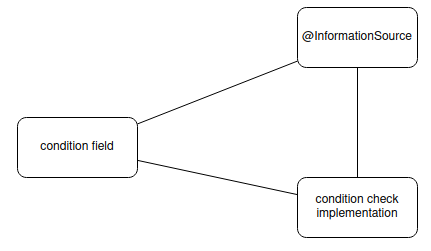
\includegraphics[width=0.75\linewidth]{./figures/condition-triplet-pattern}
    \caption{Generic illustration of the triplet pattern}
    \label{fig:condition-triplet-pattern}
\end{figure}

Adding a new condition type to the condition predicate of \RL requires the implementation of what I call the condition triplet pattern.

\paragraph{Condition Field}
Each condition type requires a meaningful keyword with a proper data type in the rule language schema.
Generally speaking, complicated condition features tremendously reduce user-friendliness.
Feedback from Dr. Bojko has shown that many simple condition fields are preferable to fewer, more complex ones, as the latter are more prone to errors.
A rule of thumb is to use flag-like boolean type fields whenever possible.

\paragraph{Information Source}
Each condition subscribes to one or more information sources.
An information source is a type of medical or administrative information that, as part of my research, I have identified as relevant for billing.
Billing-relevant information is information upon which the codes we want to derive depend.
Each Information source requires a fetch implementation, that fetches the data from other \AV services and makes sure the condition check implementation has access to it.

\paragraph{Condition Check Implementation}
Each condition field requires an actual condition implementation that expects a \code{RuleEvaluationInput} object as an input and returns the condition result.
\code{RuleEvaluationInput} objects are data classes that conveniently provide the data that represents fetched information sources required by the existing condition fields.
Section \addref describes them in more detail.

Figure \ref{fig:condition-triplet-pattern-instance-1} and \ref{fig:condition-triplet-pattern-instance-2} illustrate concrete implementations of the condition triplet pattern
for the condition fields \code{newBorn} and \code{minPatientAge}.
Both subscribe to the \code{@InformationSourcePatientAge} information source but have different condition check implementations.

\begin{figure}
    \centering
    \begin{subfigure}[b]{0.45\linewidth}
        \centering
        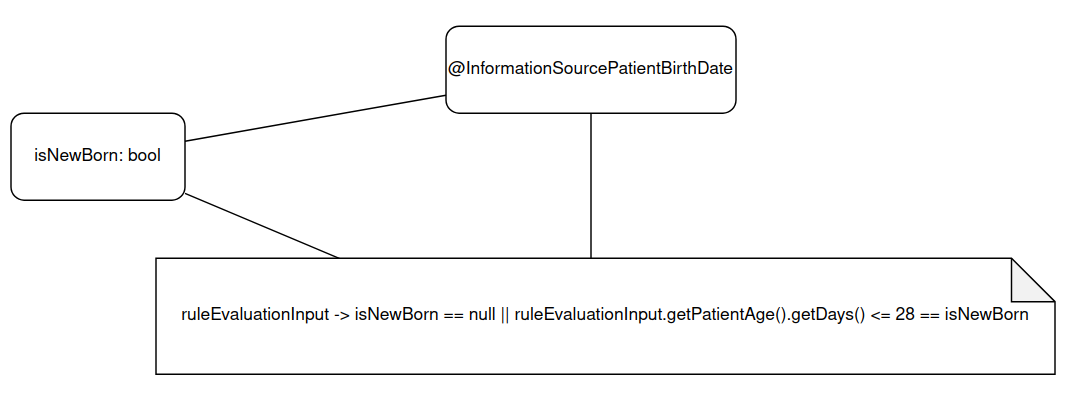
\includegraphics[width=\linewidth]{./figures/ctp-is-new-born}
        \caption{Condition Triplet pattern instance 1}
        \label{fig:condition-triplet-pattern-instance-1}
    \end{subfigure}
    % Adjust or remove the space between figures as needed
    \hspace{5mm} % This adds a bit of horizontal space between the figures
    \begin{subfigure}[b]{0.45\linewidth}
        \centering
        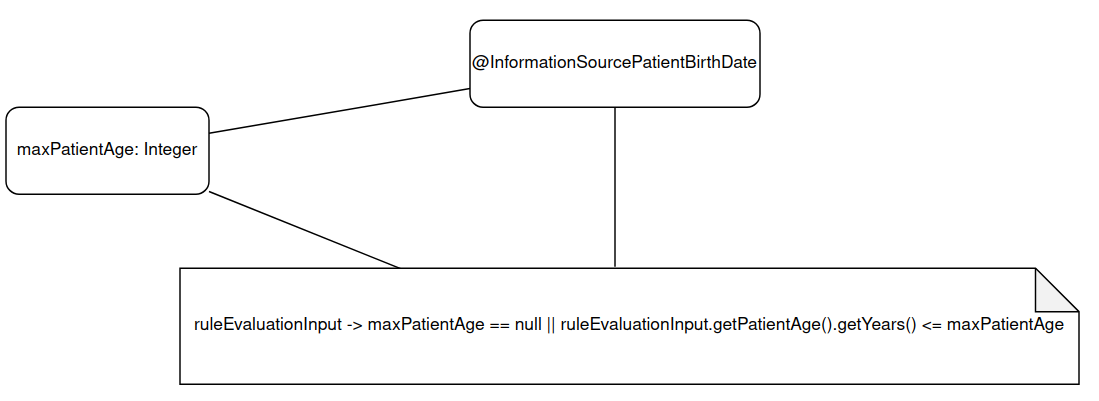
\includegraphics[width=\linewidth]{./figures/ctp-max-patient-age}
        \caption{Condition Triplet pattern instance 2}
        \label{fig:condition-triplet-pattern-instance-2}
    \end{subfigure}
    \label{fig:coffee}
\end{figure}
This section discusses the \code{condition} field of a rule.
Its value is a condition object with the following fields.

\subsection{Patient Related Conditions}\label{subsec:patient-related-conditions}

\paragraph{minPatientAge / maxPatientAge}
\code{minPatientAge} and \code{maxPatientAge} are integer fields that enable restrictions on the patient age.
Both fields store a number of years.
You can combine both to require the patient age to be within a certain age interval.

In medical practice, the age of a patient can significantly influence the complexity of a treatment.
In cases involving very young or very elderly patients, practitioners may encounter patient age specific challenges.
Due to these challenges, treatments may require more time, special care or other additional resources.
As a result, practitioners may apply billing multipliers to compensate for the additional effort.
This is why you can use the \code{minPatientAge} and \code{maxPatientAge} fields implement these types of multiplier justification rules.
There are also concrete GOÄ codes such as \goa{K1} and \goa{K2} that require the patient age.
The patient age is also highly relevant for various EBM codes, but already exists as structured conditions in the EBM catalog.
This is why using patient age conditions in EBM rules is redundant.
The information source for these two conditions is \code{@InformationSourcePatientAge}.

\paragraph{isNewBorn}
\code{isNewBorn} is syntactic sugar and a special case of the \code{maxPatientAge} condition.
It is a bool field that denotes whether a patient must be a newborn or not.
According to the GOÄ, babies that are at most 28 days old are newborns \cite{bruck1998kommentar}.
It is relevant for \goa{25: Initial newborn examination – if necessary including advice from the caregiver(s) –}, which is essentially a provision of a physical examination for newborns.
It can also be interesting for multiplier justifications.
The information source for these two conditions is \code{@InformationSourcePatientAge}.

\paragraph{patientSpeaksGerman/patientSpeaksEnglish}
\code{patientSpeaksGerman} and \code{patientSpeaksEnglish} are both boolean fields that denote whether the patients are able to communicate in the respective language.
Communication problems can increase the effort and time a treatment may require and are often used as justifications for multipliers which compensate for that.
\goa{4: taking a third-party medical history} covers an anemnesis that \todo{finish}
\code{patientSpeaksGerman} and \code{patientSpeaksEnglish} subscribe to the information source \code{@InformationSourcePatientLanguages}.

\paragraph{gender}
The \code{gender} condition is one of the most important condition types.
It is relevant for various EBM and GOÄ codes.
Similarly to patient age, gender conditions are already a structured part of the EBM catalog and do not need to be used in EBM rules.
\goa{27}, \goa{28},  GOÄ codes in section \mete{H}, Obstetrics and Gynecology, and GOÄ codes in \mete{Urology} are gender-specific.
Rules implementing these codes can use the \code{gender} condition.
It supports the string values \code{\"female\"}, \code{\"male\"} and \code{\"diverse\"}.
\code{gender} subscribes to the information source \code{@InformationSourcePatientGender}.


\paragraph{isPregnant}
The \code{isPregnant} condition is syntactic sugar for a specific case of the \code{requiredAnamnesisBlocks}
The following rules are equivalent.

\lstinputlisting[
    language=json,
    style=json,
    caption={\code{isPregnant} rule},
    label={lst:is-pregnant}
]{code/rules/specification/isPregnant.json}

A pregnancy can be reason for additionally required care or services during a treatment that is not related to the patient's pregnancy.
This is why it can be useful in multiplier justification rules.
It is also useful for \goa{23} which is applicable for an initial pregnancy-related examination.
\code{isPregnant} subscribes to the information source \code{@InformationSourceAnamnesisBlocks}.

\paragraph{isSober}
The \code{isSober} boolean condition describes the current state of the patient during the treatment.
A patient is considered non-sober when under the influence of alcohol or addictive substances.
\code{isSober} is effectively syntactic sugar for a specific use case of the \code{requiredAnamnesisBlocks} condition.
The following rules are equivalent
\lstinputlisting[
    language=json,
    style=json,
    caption={\code{is sober} rule},
    label={lst:is-sober}
]{code/rules/specification/isSober.json}


\paragraph{minNumberOfAllergies}
\code{minNumberOfAllergies} is a field that specifies the minimal number of allergies a patient requires.
From medical experts at \AV I have learned that a high number of allergies can make treatments more challenging for several reasons:
\begin{itemize}
    \item It may reduce the number of medical options as medications contain allergens or can produce them in specific environments.
    \item It can increase the complexity of the diagnostic process, as allergy reactions can mimic symptoms of other diagnoses.
    \item Patients with a high number of allergies require increased caution and care.
    Practitioners need to spend more time for history review and patient monitoring.
\end{itemize}
This makes \code{minNumberOfAllergies} a useful condition for multiplier justifications.
It subscribes to the information source \code{@InformationSourcePatientAllergies}

\subsubsection{Block Content Related Sub-rules}

A medical treatment consists of multiple stages of patient care.
Each stage has its specific aims and tools.
Anamnesis,
physical examination and procedures represent different stages of patient care and are highly relevant for billing.

\paragraph{Anamnesis}
Anamnesis is the first stage of a treatment.
Its purpose is to collect a detailed medical history from the patient\cite{lino2021medical}.
More specifically, it is about understanding the patient's general health conditions,
their lifestyle and previous patients' diagnoses.
If possible, the practitioner reviews available medical records,
interviews the patient directly or using a questionnaire\cite{zhang2011anamnevis}.

\paragraph{Physical Examination}
Anamnesis is followed by the Physical Examination.
In this practical stage, the practitioner assesses the current patient's conditions,
looking for further information about the patient's issues\cite{seidel2010mosby}.
The practitioner decides based on patient's symptoms which exact examinations are conducted.
Common examinations are checking of vital sings like blood pressure, pulse and temperature.

\paragraph{Procedures}
The procedure stage contains the actual patient-specific interventions that \todo

\paragraph{Block Contents}
As part of the Anamnesis, Physical Examination and Procedures stage,
the practitioner enters medical treatment specific information into the \AVS.
All three stages have separate documentation with a tree-like structure consisting of sections, cards and blocks.
Blocks are topic-related medical questionnaires that, depending on the patient's condition, the practitioner selects and fills out.
For example, the physical examination contains the section \mete{abdomen} that contains the \mete{liver} card.
The \mete{liver} card contains the blocks \mete{liverPalpation} and \mete{liverSize}.
Blocks are essentially small questionnaires for the practitioner with input fields to be filled out by the practitioner.
They play a huge role in treatment documentation and contain relevant medical information specific to this provided examination, procedure or anamnesis.
\code{LiverPalpation} is an example for an example for a physical block in the \code{liver} section.
A classic liver palpation examination involves answering the following questions \cite{wolf1990evaluation}:
\begin{itemize}
    \item Is the liver palpable?
    \item Is the liver texture soft or tender?
    \item Is the liver surface smooth or knotty?
    \item Is tenderness present?
    \item Are pulsations present?
    \item Is a hepato jugular reflux present?
\end{itemize}
Within the \AVS each block consists of meta-data such as timestamps, ids as well as a block content sub-object.
The \AVS defines several hundreds block contents for physical examination, anamnesis and procedures blocks.
It uses the object-relationship-mapping Hibernate to map all block content class definitions to database tables.
Each attribute of that class stores a questionnaire input entered by the practitioner.
Additionally, for each entity, there is a protobuf message definition enabling transmission of block content data from one service
to another one.
The protobuf messages of the block contents are the most important part of the structured data provided by \AV which the billing framework heavily relies on.
The protobuf message of \code{LiverPalpationMsg} looks like this:
\lstinputlisting[
    language=protobuf2,
    style=protobuf,
    caption={LiverPalpation protobuf messages}
]{code/proto/liverPalpation.proto}


The exact principle applies throughout the procedure and anamnesis stage as well.
A crucial part of the rule language is not only to check for present blocks in the treatment
but also to look inside the blocks and check for field values.
A GOÄ code might have as a condition that a liver palpation examination is part of the treatment and
the liver turned out to be palpable.
Or an OPS code should only be derived if a \code{ECG} procedure was provided and the
input field \code{telemetricExamination} inside its block has the value\true.
Logical combinations of such single field conditions may also occur.
Expressing such conditions in a well-defined and user-friendly way is an important requirement for the rule language.

\paragraph{Block Content Field Types}
A block content can contain information of different input types.
The billing framework must handle and validate each input type differently.
The most basic field types are boolean flags and numeric inputs.
The \AVS uses the following scalar wrapper protobuf messages for them:

\lstinputlisting[
    language=protobuf2,
    style=protobuf,
    caption={Scalar wrapper types}
]{code/proto/scalarWrapper.proto}

The purpose of wrapping scalars in custom protobuf messages is to make scalar default values distinguishable from missing data.
Initializing a protobuf message without explicitly setting the value of field has the consequence that the field gets initialized with its default value.
The default value for \code{int32} is 0.
If a gRPC server receives a protobuf message with an \code{int32} field set to 0, it does not know if the field was purposely initialized with 0 or not set at all.
Wrapping integers in \code{Int32W} messages makes this distinguishable.

Liver tenderness can either be present or not, which makes it a \code{BoolW} field.
The \AVS uses enumeration fields for inputs that have a limited number of predefined values
For example, the most frequently used enum type is \code{AbnormalitiesExaminationResult}.
It denotes the result of a specific examination, which can be either conspicuous or inconspicuous.

\lstinputlisting[
    language=protobuf2,
    style=protobuf,
    caption={\code{AbnormalitiesExaminationResult}}
]{code/proto/enum.proto}

Knowledge inputs are another important input type.
They serve similar purposes as enum types but are not hard-coded into the code base.
The system fetches them from a dedicated microservice that stores them in a MeiliSearch database.
Block content conditions are a powerful tool to make codes dependent on concrete medical information from anamnesis,
physical examination and procedures.

\todo{introduce nested objects, list objects}

\subsubsection{Time Related conditions}

\paragraph{procedureDurations}
Procedure durations are a crucial information source on which GOÄ codes as well as multiplier justifications rely on.
Anesthesia services such as \goa{460}, \goa{462}, \goa{473} and \goa{476} have a duration condition.
Procedures that took longer than expected are an important justification for billing multipliers.

\RL implements procedure duration conditions in a slightly different way compared to other condition fields.
Figure \ref{lst:min-max-duration} illustrates example usages of this feature.

\lstinputlisting[
    language=json,
    style=json,
    caption={\code{minDuration} and \code{maxDuration}},
    label={lst:min-max-duration}
]{code/rules/specification/minDuration.json}

Code \code{1} holds if the laryngoscopy takes at most 10 minutes.
Code \code{2} holds if the laryngoscopy takes between 10 and 20 minutes.
Code \code{3} holds if the laryngoscopy takes at least 20 minutes.

Both \code{\$minDuration} and \code{\$maxDuration} are fields that belong inside the procedure block object of the \code{requiredProcedureBlocks} field.
They start with a \"$\" sign character to mark them as special fields distinguishing them from ordinary procedure block content fields.
They are integer fields that denote a number of minutes.
A duration condition always refers to an existing procedure, which is why we write it directly into the respective procedure block condition.

\paragraph{isOutsideOfOfficeHours}
\code{isOutsideOfOfficeHours} is a boolean field that, if set to true, only evaluates to true if the treatment starts outside an official office hour.
Office hours are official time slots where practitioners provide medical services.
However, unanticipated urgencies and scheduling issues can be the reason for treatments provided outside of official office hours.
\goa{A}, \goa{B} and \goa{C} are a few examples for surcharges that apply in those cases.
This condition subscribes to \code{@InformationSourceTreatmentDate} and \code{@InformationSourceOfficeHours}.

\paragraph{daysOfWeek}
\code{daysOfWeek} is a list type condition that allows to set conditions on the week day.
Possible values inside the list are \code{\"monday\"}, \code{\"tuesday\"}, \code{\"wednesday\"}, \code{\"thursday\"}, \code{\"friday\"}, \code{\"saturday\"} and \code{\"sunday\"}.
Using any value outside of the weekdays leads to an error.
This condition is relevant for multiple GOÄ surcharges.
\lstinputlisting[
    language=json,
    style=json,
    caption={\code{minDuration} and \code{maxDuration}},
    label={lst:days-of-week}
]{code/rules/specification/daysOfWeek.json}
Code \code{1} holds if the treatment takes place on Sunday or Saturday.
The \code{daysOfWeek} condition subscribes to \code{@InformationSourceTreatmentDate}
This condition subscribes to \code{@InformationSourceTreatmentDate}.

\paragraph{timeOfDayRestrictions}
Using the \code{timeOfDayRestrictions} condition allows you to specify that the treatment should commence within any specified timeslot from a provided list of daily timeslots.
\lstinputlisting[
    language=json,
    style=json,
    caption={Code \code{1} holds if the treatment starts between 8 pm and 10 pm or between 6 am and 8 am},
    label={lst:time-of-day-restriction}
]{code/rules/specification/time-of-day-restrictions.json}
This condition subscribes to \code{@InformationSourceTreatmentDate}.

\subsection{Medical Coding Related Conditions}

\paragraph{minNumberOfDiagnosesInCurrentTreatment}
This field specifies the minimal number of diagnoses specified in this treatment.
One of the commonly used
In my research, I have learned that multimorbidity is a commonly used multiplier justification in the LMU dermatology.
Multimorbidity in medical terms defines the combination of two or more chronic medical conditions in an individual \cite{Reste2013The}.
These medical conditions may be can be a chronic disease, biopsychosocial factor or a somatic risk factor.
\code{minNumberOfDiagnosesInCurrentTreatment} is useful for implementing the multimorbidity multiplier justification rule.
The information source for this condition is \code{@InformationSourceTreatmentDiagnoses}.

\paragraph{requiredIcdCodes}

Icd codes are a highly important condition type.
They play an important role for flatrates, GOÄ codes and EBM codes.
To provide maximal flexibility, I implemented the concept of a logical code matching trees.

\lstinputlisting[
    language=json,
    style=json,
    caption={Logical Code matching tree rules},
    label={lst:logical-code-matching-tree}
]{code/rules/specification/codeMatchingTree.json}

Firstly, we define the term \"match\":
Let \( s_1 \) and \( s_2 \) be strings.
We say \( s_1 \) matches with \( s_2 \) if and only if \( s_2 \) is a prefix of \( s_1 \).
\begin{equation}\label{eq:matching}
    s_1 \text{ matches with } s_2 \iff \exists k \in \mathbb{N} \cup \{0\} : s_1 = s_2[0:k]
\end{equation}

Code \mete{1} holds if the current treatment has an ICD10 diagnose that matches with \mete{B20}.
Rule \mete{2} makes use of the logical \code{OR} operator and holds if the current treatment has a diagnose that matches with \mete{R07.0}, \mete{R07.1} or \mete{L}.

Note that \mete{L} is not a ICD code but chapter within the ICD catalog.
According to the definition \ref{eq:matching}, \mete{L} matches with every single ICD10 code in the \mete{L} chapter as all of them have the prefix \"L\".
This makes it easy to specify a large group of ICD10 codes in a logical code matching tree.
The ICD10 catalog has a tree structure that maintains the invariant that each node is a prefix of its child nodes.
In other words, each node matches its parent node.
Nested nodes are chapters, sections and subsections.
Leaf nodes are actual ICD10 codes.

Note the code range \mete{R47..R49} used in rule \mete{3}.
This indicates a discrete interval of codes between \mete{R47} and \mete{R49}, including both borders.
\mete{R47..R49} includes all codes that match with \mete{R47}, \mete{R48} and \mete{R49}.

Just as \code{minNumberOfDiagnosesInCurrentTreatment} it subscribes to the information source \code{@InformationSourceTreatmentDiagnoses}.
The practitioner manually selects diagnoses for the treatment.
This is why diagnoses are part of the treatment object and are straight-forward to fetch.

\paragraph{requiredOpsCodes}

\code{requiredOpsCodes} is equivalent to \code{requiredIcdCodes}, but applies to OPS codes.

The major difference here is how the system fetches OPS codes for this treatment.
Unlike diagnoses, the practitioner does not manually select OPS codes for the conducted procedures.
The billing experts at \AV have therefore requested that the billing framework should automatically derive OPS codes for treatments.
I solved this by defining OPS rules as a new rule type.
Any rule componenent that needs to derive OPS rules makes use of another rule component, namely \code{OpsRuleComponent}.
It implements data fetching for \code{InformationSourceOpsCodes} by deriving OPS codes using OPS rules.
Just as any rule type, billing experts are responsible for writing OPS rules, as well.

\paragraph{requiredTargetCode}

\code{requiredTargetCode} is similar to \code{requiredOpsCodes} and \code{requiredIcdCodes}, but has a few differences.
Firstly, it refers to the result set of the derivation.
Using this condition, you can implement that a code can only be billed with another set of codes.
Billing experts need this feature to implement \goa{K1} and \goa{K2} as well as other surcharge codes in the GOÄ.
Secondly, it defines the term \"match\" as a direct string equality.
\begin{equation}\label{eq:matching-string-equals}
s_1 \text{ matches with } s_2 \iff s_1 = s_2
\end{equation}
GOÄ, EBM and other possible code systems do not offer a hierarchical prefix tree structure that would allow definition \ref{eq:matching}.
Instead, \code{requiredTargetCode} uses definition \ref{eq:matching}.
Section \addref offers a more detailed description of how the condition checking for \code{requiredTargetCode} actually works.

\subsection{Previous Occurrence related Conditions}\label{subsubsec:previous-occurrence-related}

The \AVS internally structures treatments as follows:
A patient multiple billing cases, each one representing a quarter of the year.
During a quarter, a patient may have multiple visits.
Each visit has a reference to the respective billing case.
During a visit, a patient can have one or more treatments.
For example, a patient can have an operation followed by a medical round.
A medical round is a part of hospital routine where healthcare professionals visit patients at their bedsides,
assess the patient's medical condition and evaluate the treatment process.
The \AVS considers the operation and the medical round both as treatments linked to the same visit.
The smallest units in the hierarchy are the billing positions that are attached to a treatment.

Another important context within the private billing is the so-called treatment case.
A treatment case refers to the month following an initial treatment for a new medical condition \cite{bruck1998kommentar}.
Treatment cases can run in parallel if a patient has two unrelated medical conditions.
For example, if a patient visits the doctor for a knee injury on the 4th of May, a new treatment case starts for this knee injury and lasts until the 5th of June.
Every treatment related to this knee injury between the 4th of May and the 5th of June belongs to this treatment case.
If the patient visits the same doctor for a viral infection on the 10th of May, a second treatment case begins, lasting until the 11th of June.
Two treatment cases run in parallel because both medical conditions, the knee injury and the viral infection, are independent.
A treatment case always spans one month.
This is why if the patient receives treatment related to the knee one month after the initial treatment, a separate treatment case starts, even though both treatments are related to the same diagnosis.

Occurrence related condition types do not subscribe to any information source.
They do not require information from an external service but rely on the billing history of the patient.
The billing service stores billing positions in the local database.
Evaluating each of the following conditions includes a query on the

\paragraph{maxAmountPerBillingCase / maxAmountPerTreatmentCase / maxAmountPerVisit / maxAmountPerTreatment}
These condition fields set a limit on the code occurrences in the respective context.
The code is always the conclusion of the rule the condition is part of.
\todo{add example}


\paragraph{maxAmountPerDay / maxAmountPerMonth / maxAmountPerYear}
Similarly to the previous condition fields, \RL also allows setting limits for code usages in specific time spans.
\todo{add example}


\paragraph{onlyOncePerGoaeTreatmentCaseInCombinationWithSpecialServices}
This boolean condition field handles a highly specific but important edge-case involving \goa{1} and \goa{5}.
From the \PVC seminar, I have learned that within the same treatment case, both codes can be billed in combination with a special GOä code at most once.
A special GOÄ code is a code whose numeric number is higher or equal to 200.
This means within the same treatment case \goa{1} can be billed as often as possible, but only once in combination with any code larger than 200.
The same holds for \goa{5}.

\subsection{Service Performer related Conditions}

\paragraph{performerIsDoctor}
The \code{performerIsDoctor} condition is a boolean condition field that allows to impose conditions on the practitioner type.
The current version of the \AVS supports the following practitioner types:

\lstinputlisting[
    language=protobuf2,
    style=protobuf,
    caption={\code{AbnormalitiesExaminationResult}},label={lst:AbnormalitiesExaminationResult}]{code/proto/roleTypes.proto}

Given the rules in code snippet \ref{lst:performerIsDoctor}, \code{code1} would hold if the practitioner had the role \code{ROLE\_TYPE\_DOCTOR}
or \code{ROLE\_TYPE\_HEAD\_DOCTOR}.
Otherwise, \code{code2} would hold.
This condition is relevant for \goa{1} and \goa{2}, which are only applicable by doctors.

\lstinputlisting[
    language=protobuf2,
    style=protobuf,
    caption={\code{AbnormalitiesExaminationResult}},
    label={lst:performerIsDoctor}
]{code/rules/specification/performerIsDoctor.json}

\subsection{Conflict Conditions}\label{subsec:conflict-conditions}
Conflict conditions are special fields that the framework cannot evaluate during the ordinary rule evaluation phase.
The reason for that is the these fields require the final rule evaluation set as an input, which is obviously not known during the rule evaluation phase.
The framework does not define a information source for this type of information.
Instead, these fields receive a special handling in a separate derivation stage described in section \addref.

\paragraph{singleBillingPosition}
\code{singleBillingPosition} is a special condition type that if set to \true only evaluates to \true if it is the only code in the derivation result.
It is relevant for \goa{3}.
This condition does not subscribe to any information sources.

\paragraph{singleBillingPositionIfPractitionerIsDoctor}
\code{singleBillingPositionIfPractitionerIsDoctor} is an extension of of \code{singleBillingPosition}
This admittedly highly specific boolean condition field behaves as follows:

\[
    \code{\{singleBillingPositionIfPractitionerIsDoctor : true\} = \true} \leftrightarrow \code{\{practitionerIsDoctor : true\} = \false} \land \code{\{singleBillingPosition : true\} = \true}
\]


This condition subscribes to \code{@InformationSourcePractitionerType}.


\todo{finish this}

Even though this condition  condition field is admittedly very specific

that if set to true only evaluates to \true if it is the code in the derivation result.
It evaluates to true if the practitioner is not a doctor or the conclusion code is the only code in the derivation result.
This condition field requires special handling but also subscribes to information source \code{@InformationSourcePractitionerType}.

\paragraph{excludedCodes}
This condition field expects a list of conclusions as a value.
A rule using the \code{excludedCodes} field evaluates to false if any code in the \code{excludedCodes} list is a derivation result.
This


\subsection{Miscellaneous Conditions}\label{subsec:miscellaneous-conditions}

\paragraph{isCareRound / isMedicalRound}
\code{isCareRound} and \code{isMedicalRound} are boolean conditions that enable you to check if the treatment is a care / medical rounds.
\goa{46}, \goa{48} and \goa{50} are a few examples for services that require that information.
Both fields subscribe to the information source \code{@InformationSourceTreatmentType}


\subsection{Quantity Functions}\label{subsec:quantity-functions}

In the previous chapter we introduced the concept of a billing rule.

Not only which codes are part of the billing but also their quantity is highly important information.
In the previous section, we explained how the billing framework derives a set of applicable billing codes.
The result data type was essentially a set of billing codes.
In this section, we generalize the framework in such a way that it returns each code in combination with its quantity.

We extend the general rule structure by introducing the concept of quantity functions.
Similarly to rule conditions, quantity functions are evaluatable subcomponents of a rule.
The framework evaluates quantity functions of rules for a\code{RuleEvaluationInput}.
The result is an integer that indicates how often it should be billed in the billing.

\begin{equation}
    \label{eq:quantity-function-natural}
    f_{quantity}: \code{RuleEvaluationInput} \longrightarrow \mathbb{N}
\end{equation}

Billing code quantities typically rely on two types of billing information.
Subsection\ref{subsubsec:quantity-derivation-from-procedure-information} and\ref{subsec:quantity-derivation-from-durations} explain these sources.

\subsubsection{Quantity Derivation From Procedure Information}\label{subsubsec:quantity-derivation-from-procedure-information}

I derived the requirement for quantity functions from \goa{255: Injection, intra-articular or perineural}.
It is an example of a code, that is likely to appear in a billing with a quantity larger than one.

The so-called Spine Infiltration is a procedure, that includes injections into spine nerves.
Billing experts use \goa{255} for this medical service.
Procedure block \code{SpineInfiltrationMsg} represents this procedure.
However, \goa{255} typically applies once for each spine injection the practitioner actually provided.
Therefore, a spine infiltration can include multiple injections at different localizations.
The system should not only be able to derive \goa{255} for a provided spine infiltration, but should also be able to derive the correct quantity of \goa{255} codes.

To illustrate this example, it is worth mentioning that the human spine consists of three primary regions \cite{BOGDUK2016675}:
\begin{itemize}
    \item The cervical spine, the thoracic spine, and the lumbar spine.
    The cervical spine comprises the uppermost part of the spine, which is the neck and head.
    \item The thoracic spine, located in the middle, has twelve vertebrae attached to the rib cage, providing stability and structure to the upper body.
    \item Lastly, the lumbar spine at the lower back is made up of five larger vertebrae, designed to bear the body's weight and provide flexibility and movement.
\end{itemize}
Each region has well-defined localizations that can be targets for injections.
The \AVS stores the data of a spine infiltration in a \code{SpineInfiltrationMsg}procedure block.

The following code snipped displays a simplified version of it.
\lstinputlisting[
    language=protobuf3,
    style=protobuf,
    caption={Relevant localizations in a spine infiltration}
    label={lst:spineInfiltration},
]{code/proto/spineInfiltration.proto}


\code{SpineInfiltrationMsg} has a nested message\code{NerveRootBlockMsg}.
\code{NerveRootBlockMsg} contains the messages,\code{CervicalSpineMsg}\code{ThoracicSpineMsg} and\code{LumbarSpineMsg}.
These messages represent the before-mentioned sections of the human spine.
Each variable in these nested messages is of type \code{Laterality}and represents injections at the respective localization alongside the spine.
The laterality of an injection refers to the specific side or sides where the injection is administered in the spine localization.
This can be either on the left side, the right side, or on both sides.

To get the total number of injections, the system would need to peek into the nested messages \code{CervicalSpineMsg}, \code{ThoracicSpineMsg} and\ code{LumbarSpineMsg} and compute the total number of injections from the laterality values.
Additionally, the framework needs to be able to understand that \code{LATERALITY\_NONE} refers to zero and \code{LATERALITY\_LEFT} as well as\code{LATERALITY\_RIGHT} refer to one injection.
\code{LATERALITY\_BOTH} refers to two injections.
It is important to assign quantities to enum values.


\subsubsection{Quantity Derivation From Durations}\label{subsec:quantity-derivation-from-durations}

Many GOÄ codes specify not only a service content but also a time range.
If provided services exceed that time range the respective code can be billed more than once.

\goa{21: Incoming human genetic counseling, per commenced half-hour and session} is an example for such a code.
If the counseling takes one hour and 10 minutes, \goa{21} can be billed 3 times.
Similar codes are \goa{61: Assistance in the medical service of another doctor (Assistance), per commenced half-hour}
and \goa{85: Written expert opinion involving an effort exceeding the usual extent – possibly with scientific justification –, per commenced hour of work}
Codes that with that characteristic often end with \("\)per commenced hour\("\) or \("\)per commenced half-hour\("\) to indicate the time range.
Those are comparably simple cases.

\mete{Section D: Anesthesia Services} contains a specific class of edge case that use time ranges.

\goa{462: Combined anesthesia with endotracheal intubation, up to one hour} and \goa{463: Combined anesthesia with endotracheal intubation, each additional commenced half-hour}
both denote the same procedure provided, but as their names suggest, they distinguish between different periods of service provision.
\goa{462} is applicable only once per procedure.
On the other hand, code \goa{463} covers each additional half-hour beyond the initial hour.
Its billing number is variable and depends on the total duration of the anesthesia.
\goa{463} excludes the first hour of service provision, already covered under code \goa{462}.

The GOÄ distinguishes between \goa{462} and \goa{463} because of the following reasons.
\goa{462} covers both the induction and the maintenance of anesthesia for the first hour.
This is the most critical phase involving continuous administration of medication to make sure the patient remains asleep.
The time after the first hour typically requires only maintenance of anesthesia and is therefore less critical.
\goa{463} applies to subsequent commenced half-hours after the first hour and is therefore lower priced than \goa{462}.


Anesthesia services frequently use this pattern of code groups referring to the same provided procedure but distinguishing between service periods.
Equivalent examples are \goa{460/461}, \goa{476/477} and \goa{478/479}.
\goa{473, 474 and 475} are a more special example.
They refer to an initiation and monitoring of a continuous subarachnoid spinal anesthesia, again distinguishing between durations.
\goa{473} applies to durations shorter than five hours, \goa{474} to the subsequent five hours and \goa{475} applies once for the second and every subsequent day.

These examples lead to concrete requirements for the billing framework and underline the importance of \"quantity functions\".
They must be expressive enough to represent and manage the nuances of these examples.
Section\ref{sec:quantity-function-specification} illustrates how users can express these cases using the rule language.

\subsection{Partial Billing Quantitys}\label{subsec:partial-billing-quantitys}
In very special cases billing codes apply with a reduced quantity of points.

%There are at least two cases:
%\goa{D} is a surcharge for services provided on saturday, sunday and on holidays.
%If service provision happens during an opening hour, \goa{D} only applies with half the fee, though.
%This is also the case for surcharges \goa{E}, \goa{F}, \goa{G} and \goa{H} if \goa{51} is part of the billing, as well.
%
%The framework must be able to express these edge cases but does not allow any point value manipulations of billing codes.
%It solves this issue using quantity functions.
%In those cases the quantity function must be able to evaluate to 0.5 which results in the same fee reduction as required by the GOÄ specification.
%
%This requirement changes the formal definition given in formula \ref{eq:quantity-function-natural} to:
%\begin{equation}
%    \label{eq:quantity-function-real}
%    f_{quantity}: \code{RuleEvaluationInput} \longrightarrow \mathbb{R}^{+} \\ \left{0\right}
%\end{equation}
%Quantity function now evaluate


\subsection{The Multiplier Function}\label{subsec:the-multiplier-function}
The multiplier justification rule type does not use the concept of a quantity.
They require \code{condition} blocks to make them derivable for certain conditions.
Additionally, we also want to compute suggested multiplier values dynamically from the environment.
This is why I introduced the \code{multiplier} field, which is very similar to the previously introduced \code{quantity} field.
Both make use of numeric function expressions that allow for dynamic computation from their environment.

In contrast to quantity functions, a multiplier expression returns a positive floating point number with two decimal places.

In this subsection, we illustrate this concept using the following example.
From Dr. Sahra Bojko I have learned that regular laryngoscopies should take at most 20 minutes.
We can apply a duration related multiplier for laryngoscopies that exceed this duration.
The longer the laryngoscopy takes, the greater should be the value of the multiplier for the provided service.
One way of implementing this is by declaring multiple multiplier justification rules applying to different time intervals.

\clearpage
\lstinputlisting[
    language=json,
    style=json,
    caption={Step multiplier function},
    label={lst:multiplier-justification-function-steps}
]{code/rules/specification/multiplier-expression-steps.json}

All three rules logically exclude themselves due to the duration intervals in their \code{laryngoscopy} block conditions.

This implements the following step function declared in equation \ref{eq:multilier-justification-step-function} and illustrated in figure \ref{plot:multiplier-justification-step-function}.

\begin{equation}\label{eq:multilier-justification-step-function}
    f(x) =
    \begin{cases}
        1.5 & \text{for } 20 \leq x < 30, \\
        2.5 & \text{for } 30 \leq x < 40, \\
        3.5 & \text{for } x \geq 40.
    \end{cases}
\end{equation}

\begin{center}
    \label{plot:multiplier-justification-step-function}
    \begin{tikzpicture}
        \begin{axis}
        [
            axis lines=middle,
            xlabel={duration in minutes},
            ylabel={suggested multiplier value},
            xmin=0, xmax=70,
            ymin=0, ymax=4,
            xtick={10,20,30,40,50,60},
            ytick={0,1,2,3,3.5},
            clip=false,
            domain=20:75,
            samples=100,
        ]
            \addplot+[no marks, blue, thick, const plot] coordinates {(20,1.5) (30,2.5) (40,3.5) (70,3.5)};
        \end{axis}
    \end{tikzpicture}
\end{center}

Another more compact way to implement this is using a single rule with a more sophisticated multiplier expression.
Formula \ref{eq:bounded-linear-multiplier-function} is a valid choice for a multiplier function.

\begin{equation}
    \label{eq:bounded-linear-multiplier-function}
    f: \left[20, \infty\right) \rightarrow \left[ 1, \infty \right) : d \mapsto \min\left( 3.5, \frac{5}{40} d - \frac{3}{2} \right)
\end{equation}


Code snippet \ref{lst:multiplier-justification-function-linear} illustrates a rule that implements this multiplier function.
Note that the \code{condition} assures that the rule only applies to treatments with a provided laryngoscopy that took at least \code{20} minutes.
This sets the domain of the function to $\left[20, \infty\right)$.
This way inside, we can inside the \code{multiplier} block safely assume that the duration is greater or equal to 20.

\lstinputlisting[
    language=json,
    style=json,
    caption={Bounded linear multiplier function},
    label={lst:multiplier-justification-function-linear}
]{code/rules/specification/multiplier-expression-linear.json}


\begin{center}
    \begin{tikzpicture}
        \begin{axis}
        [
            axis lines=middle,
            xlabel={duration in minutes},
            ylabel={suggested multiplier value},
            xmin=0, xmax=70,
            ymin=0, ymax=4,
            xtick={0,10,20,30,40,50,60,70},
            ytick={0,1,2,3,3.5,4},
            clip=false,
            domain=20:75,
            samples=100,
        ]
            \addplot+[no marks, blue, thick] {min(5/40*x - 1.5, 3.5)};
        \end{axis}
        \label{plot:linear-mul-just}
    \end{tikzpicture}
\end{center}

Plot \ref{plot:linear-mul-just} illustrates the graph for the multiplier function.

For ordinary laryngoscopies that take less than 20 minutes, the multiplier justification rule does not match at all.
Note that with increasing laryngoscopy duration, the suggested multiplier linearly increases between 20 and 40 minutes.
For very unlikely cases where complications are so severe that the laryngoscopy takes more than 40 minutes, the rule suggests the maximum multiplier value of 3.5.


\subsection{The Target Code Field}\label{subsec:the-target-code-field}
The \code{targetCode} field is a higher level code visible in code snippet visible in code snippet \ref{lst:rule-root}.
We can use it to specify a hint for the application code that the conclusion of the rule should be applied to a target.
The conclusion of the rule is always the value of the \code{code} field.

The current concrete use case for this feature are multiplier justifications.
We generally distinguish between procedure-specific and general multiplier justifications.
Procedure-specific Multiplier Justifications specify a GOÄ code in their \code{targetCode} field and are only applicable to this GOÄ code.
General Multiplier Justifications have no target.
It is the user's or the application code's responsibility to assign the Multiplier Justification to a appropriate GOÄ code.
Section \ref{subsec:multiplier-justification-rules} illustrates concrete multiplier justification rules that are part of the research results of this work.




\chapter{The Billing Optimization Framework}\label{ch:the-billing-optimization-framework}

%\section{Aspects of Rule-Based Systems}\label{sec:aspects-of-rule-based-systems}

Rule-based systems are systems that apply predefined rules to a given problem or dataset
and derive conclusions or make decisions based on the input data\cite{grosan2011rule}.
Deriving conclusions requires expert knowledge in the respective domain.
The main difference to an ordinary software system is that the system does not hard-cde the domain-specific knowledge.
Instead, we have rules that encode domain knowledge in a predefined rule language.
The system treats these rules as an external resource and loads them into a rule-base.
It directly uses the rule-encoded knowledge found in the rule-base to derive conclusions.
A rule-based systems is therefore a framework for knowledge experts that do not need to have a technical background.
However, users must possess the requisite skill to translate their expert knowledge into rules,
which requires them to have a profound understanding of the rule language.


These rules are typically explicit,
declarative and logical statements about specific conditions that must hold to make the system act in a specific way.
Rule-based systems are inherently knowledge-intensive applications\cite{hayes1985rule}.
Their performance heavily relies on the quality,
depth and richness of the domain-specific knowledge encoded in its rules.
Rules in a rule-based system have the following form:

\[
    \text{<Rule-id>}: \text{IF} \text{<condition>} \text{THEN} \text{<conclusion>} \text{holds}
\]


A rule consists of a \textbf{condition} and a \textbf{conclusion}
and makes the rule-based system apply the conclusion if the condition holds.
Its purely logical and declarative nature and makes them explicit, deterministic and predictable.
Each rule has an identifier that makes it unique among the set of all rules in the system.

However, due to their simplicity, they also come with some limitations.
They lack the ability to learn from new data autonomously and new rules to be added manually.
Domain knowledge can also change which requires domain experts to be responsible for maintenance and rule updates.
Knowledge domains can also be highly complex.
High complexities increase the number of rules that a rule-based system requires to work effectively in production.


\subsection{General Rule Language Requirements}\label{subsec:general-rule-language-requirements}

\begin{itemize}
    \item Clearly defined syntax and semantics.
    \item User-friendliness
    \item Satisfactory expressiveness for all concrete cases
    \item Rule base should be easy to extend
    \item Rule language should be updatable
\end{itemize}

As every domain-specific language, a rule language needs clearly defined semantics and syntax.


Finding the correct compromise between language expressiveness and user-friendliness\cite{https://doi.org/10.1002/widm.11} requires careful consideration.
On one side,
the language needs
to be sufficiently powerful to articulate all conditional logics and edge cases that may occur in the knowledge domain.
On the other side, the language must remain accessible to domain experts that will finally implement rules.
For the language to remain relevant and effective, it should adapt over time, incorporating feedback from its user base.
This might involve introducing new constructs or syntactic sugar to simplify common tasks.


Possible rule strategies:

<Rule-id>: IF <condition> THEN <conclusion>

A rule-based system to work its rule base needs
to contain a high number of valid rules that incorporate large parts of the respective knowledge domain.
For the sake of transparency every rule needs an id that identifies holding rules in an evaluated result set.

A condition is essentially a function which the rule engine can.

\[
    \text{conclusion holds} \Leftrightarrow f(\text{input1}, \text{input2}, \ldots, \text{input3}) = \text{true}
\]

\section{Inference Mechanism}\label{sec:inference-mechanism}

Basically, there are two modes of inference mechanisms\cite{https://doi.org/10.1002/widm.11}

\begin{itemize}
    \item forward chaining
    \item backward chaining
\end{itemize}


Forward chaining is an inference strategy where reasoning begins with the existing facts.
The inference engine simply applies the conditions of all rules in the rule base to the known data.
Finally,
we add the conclusions of those rules
whose conditions hold to the set of valid conclusions and thus to the set of facts.

Backward chaining uses a different strategy\cite{al2015comparison}.
The user specifies a single goal or hypothesis
which we want to proof or reject and looks for rules in the rule base whose conclusion would match with it.
The conditions of those rules are now the new goal which the system needs to satisfy.
The system then recursively looks for rules with matching conclusion
and tries to satisfy their conditions as new sub-goals.
If the system is able to reduce all sub-goals to facts, we accept the initial hypothesis.
If the system cannot find further rules, we reject the initial hypothesis.
This inference strategy is often used in diagnostics and decision support\cite{https://doi.org/10.1002/widm.11}

Part of the design of the rule-based framework in this work is the decision between forward and backward chaining.
Chapter \todo{add correct ref} revisits this design decision
and provides a more detailed justification for the choice taken.

%\section{Billing Relevant Information Sources}\label{sec:billing-relevant-information-sources}


Before introducing the rule language,
we need to firstly define all sources of information that are relevant for billing.
Its semantics and features were designed based on this knowledge.

Additionally,
it must be assured that the\AVS actually tracks and stores all information relevant for billing as structured data.
For that, the\AVS might require further adjustments and updates.

On one hand, the treatment documentation must contain all medically relevant data,
but now it also needs to cover billing-related information as well.


%The workflow is as follows:
%\begin{enumerate}
%    \item \Me
%    at\AV use their knowledge to define formal specifications for the anamnesis,
%    physical examination and procedures blocks.
%    This is a continuous process where requests and feedback from customers are taken into consideration.
%    \item \Se at\AV create new blocks or update existing ones according to changes in the medical specifications.
%    \item \Be at\AV with medical background,
%    an understanding of the block data models and the rule language implement formal billing rules
%    using the rule language.
%    \item At Back-End start-up the system loads the rule files into the Billing-Service
%which are then available for automated billing code derivation.
%\end{enumerate}

Firstly, we need to specify the concrete use-cases for the rule language.
The initial plan was to implement two separate languages, one for statutory billing and one for private billing.
Section\ref{sec:billing-catalogs} introduces their billing catalogs and presents their differences and characteristics.

However, collaboration with medical experts has revealed further requirements for the billing framework.
This includes additional use-cases for the billing language.
The following list contains all rule types that the framework currently supports:
\begin{itemize}
    \item GOÄ billing rules for deriving GOÄ billing codes from private treatments
    \item EBM billing rules for deriving EBM billing codes from statutory treatments
    \item OPS code rules for deriving procedure codes from treatment documentation.
    OPS codes are relevant information for both GOÄ and EBM codes as well as multiplier justifications.
    \item Multiplier Justification rules for detecting challenging conditions in private treatments
    which serve as justifications for multipliers
    \item Special Flat Rate rules
    for detecting flat rates that can be applied to billing positions in the statutory treatment
\end{itemize}

The initial idea of having separate implementations for each rule type turned out to be not very scalable.
Each rule type has a set of relevant information sources and therefore also ignores sources.
But the key point is that there are many information sources shared by multiple rule types.

For example, the patient age is highly relevant for GOÄ and EBM codes, Multiplier Justifications but not for OPS codes.
Previous allergies are relevant for Multiplier Justifications but not necessarily for GOÄ codes.
This is the reason I decided to use a single rule engine that implements all conditions used by any rule type.
Each rule type defines its own interface and re-uses the rule engine.
Therefore,
we consider each information source illustrated in this section as primarily independent of any rule type or use case.

\subsection{Information Scope}
Part of this work was
to identify billing-relevant information sources through and expert interviews and cooperation with medical experts.
From a higher level perspective, all found information sources are part of the following domains:
\begin{itemize}
    \item
    The treatment documentation that contains all medical information of the treatment whose services we want to bill
    \item Patient characteristics that are independent of the current treatment
    \item Information referring to the providing practitioner
    \item Treatment history consisting of all billing codes in previous treatments aggregated by treatment,
    visit and billing case
\end{itemize}
During the development of the billing framework, I placed great emphasis on extensibility.
Adding new condition types to the core engine and making them available to all rule types is straightforward.
The following subsections give further explanations for the most important information sources.

\subsection{Block Contents}
A medical treatment consists of multiple stages of patient care.
Each stage has its specific aims and tools.
Anamnesis,
physical examination and procedures represent different stages of patient care and are highly relevant for billing.

\subsubsection{Anamnesis}
Anamnesis is the first stage of a treatment.
Its purpose is to collect a detailed medical history from the patient\cite{lino2021medical}.
More specifically, it is about understanding the patient's general health conditions,
their lifestyle and previous patients' diagnoses.
If possible, the practitioner reviews available medical records,
interviews the patient directly or using a questionnaire\cite{zhang2011anamnevis}.

\subsubsection{Physical Examination}
Anamnesis is followed by the Physical Examination.
In this practical stage, the practitioner assesses the current patient's conditions,
looking for further information about the patient's issues\cite{seidel2010mosby}.
The practitioner decides based on patient's symptoms which exact examinations are conducted.
Common examinations are checking of vital sings like blood pressure, pulse and temperature.

\subsubsection{Procedures}
The procedures stage contains the actual patient specific interventions that \todo

\subsection{Block Contents}
During Anamnesis,
Physical Examination and Procedures the practitioner enters medical treatment specific information into the \AVS.
The data is part of the treatment documentation and critical for billing.

The documentations of all three stages are filled out by the practitioner and are structured in sections,
cards and blocks.

For example, inside the physical examination there is the section \mete{abdomen},
which contains the\mete{liver} section.
Blocks are essentially small questionnaires for the practitioner with input fields to be filled out by the practitioner.
They play a huge role in the treatment documentation
and contain all relevant medical information specific to this conducted examination,
procedure anamnesis.
One example for a physical block in the \code{liver}section is\code{LiverPalpation}.
A liver palpation involves investigating the following questions

\begin{itemize}
    \item Is the liver palpable?
    \item Is the liver texture soft or tender?
    \item Is the liver surface smooth or knotty?
    \item Is tenderness present?
    \item Are pulsations present?
    \item Is a hepato jugular reflux present?
\end{itemize}

Each of the more than 100 block contents in the \AVS are represented by a dedicated Hibernate entity classes.
Each attribute of that class stores a questionnaire input entered by the practitioner.
Additionally, for each entity, there is a protobuf message enabling transmission of block content data from one service
to another one.

The protobuf message of \code{LiverPalpationMsg} looks like this:

\lstinputlisting[
    language=protobuf2,
    style=protobuf,
    caption={LiverPalpation protobuf messages}
]{code/proto/liverPalpation.proto}

The exact principle is applied throughout all the procedures and anamnesis as well.
A crucial part of the rule language is not only to check for block content availabilities in the treatment
but also to look inside the blocks and check for conditions on fields.
A GOÄ code might have as a condition that a liver palpation examination is part of the treatment and
the liver turned out to be palpable.
Or an OPS code should only be derived if a \code{ECG}procedure was provided and the
input field\code{telemetricExamination} inside its block has the value\code{true}.
Logical combinations of such single field conditions may also occur.
Expressing such conditions in a well-defined and user-friendly way is an important requirement for the rule language.

\subsection{Block Content Field Types}
A block content can contain information of different input types.
The billing framework must handle and validate each input type differently.

The most basic field types are boolean flags and numeric inputs.
The \AVS uses the following scalar wrapper protobuf messages for them:

\lstinputlisting[
    language=protobuf2,
    style=protobuf,
    caption={Scalar wrapper types}
]{code/proto/scalarWrapper.proto}

Liver tenderness can either be present or not.
This information is thus entered in a \code{BoolW]} field.
We use enumeration fields for inputs that have a limited number of predefined values
For example, the most frequently used enum type is \code{AbnormalitiesExaminationResult}.
It denotes the result of a specific examination, which can be either conspicuous or inconspicuous.

\lstinputlisting[
    language=protobuf2,
    style=protobuf,
    caption={\code{AbnormalitiesExaminationResult}}
]{code/proto/enum.proto}

Another important input type are knowledge inputs.
They serve similar purposes as enum types but are not hard-coded into the code base.
The system fetches them from a dedicated microservice that stores them in a MeiliSearch database.
Enum field


The \AVS uses block content messages to store user inputs of medical questionnaires filled out by practitioners.

The \AVS uses this concept of blocks as a medical questionnaires storing anamnesis, physical examination and procedure
data as protobuf messages.

Block content conditions are a powerful tool to make codes dependent on concrete medical information from anamnesis,
physical examination and procedures.
They are one of multiple condition types in a rule and are called \code{BlockContentSubRules}


There is another condition
as well that are related to information outside the treatment such as general patient information,
that get

\subsection{EBM billing rules}\label{subsec:ebm-billing-rules}
As described in section\ref{sec:ebm-conditions} the Ebm catalog already contains structured,
treatment content unrelated conditions.
EBM rules therefore do not need to include them.
However, what is left are treatment-specific conditions.
Rules

\subsection{OPS code rules}\label{subsec:ops-code-rules}
OPS codes are identifiers of medical procedures.
They are completely independent of patient information and their previous medical history.
So in order to derive them automatically, they only need the procedure block as an input.

\subsection{GOÄ billing rules}\label{subsec:goa-billing-rules}


\subsection{Special Flat Rates}\label{subsec:special-flat-rates}


%\section{Rule Language Specification}\label{sec:rule-language-specification}

\subsection{The Condition Predicate}\label{subsec:the-condition-predicate}

\subsubsection{Block Content Related Sub-rules}

A medical treatment consists of multiple stages of patient care.
Each stage has its specific aims and tools.
Anamnesis,
physical examination and procedures represent different stages of patient care and are highly relevant for billing.

\paragraph{Anamnesis}
Anamnesis is the first stage of a treatment.
Its purpose is to collect a detailed medical history from the patient\cite{lino2021medical}.
More specifically, it is about understanding the patient's general health conditions,
their lifestyle and previous patients' diagnoses.
If possible, the practitioner reviews available medical records,
interviews the patient directly or using a questionnaire\cite{zhang2011anamnevis}.

\paragraph{Physical Examination}
Anamnesis is followed by the Physical Examination.
In this practical stage, the practitioner assesses the current patient's conditions,
looking for further information about the patient's issues\cite{seidel2010mosby}.
The practitioner decides based on patient's symptoms which exact examinations are conducted.
Common examinations are checking of vital sings like blood pressure, pulse and temperature.

\paragraph{Procedures}
The procedure stage contains the actual patient-specific interventions that \todo

\paragraph{Block Contents}
During Anamnesis,
Physical Examination and Procedures the practitioner enters medical treatment specific information into the \AVS.
The data is part of the treatment documentation and critical for billing.

The documentations of all three stages are filled out by the practitioner and are structured in sections,
cards and blocks.

For example, inside the physical examination there is the section \mete{abdomen},
which contains the\mete{liver} section.
Blocks are essentially small questionnaires for the practitioner with input fields to be filled out by the practitioner.
They play a huge role in the treatment documentation
and contain all relevant medical information specific to this conducted examination,
procedure anamnesis.
One example for a physical block in the \code{liver}section is\code{LiverPalpation}.
A liver palpation involves investigating the following questions

\begin{itemize}
    \item Is the liver palpable?
    \item Is the liver texture soft or tender?
    \item Is the liver surface smooth or knotty?
    \item Is tenderness present?
    \item Are pulsations present?
    \item Is a hepato jugular reflux present?
\end{itemize}

Each of the more than 100 block contents in the \AVS are represented by a dedicated Hibernate entity classes.
Each attribute of that class stores a questionnaire input entered by the practitioner.
Additionally, for each entity, there is a protobuf message enabling transmission of block content data from one service
to another one.

The protobuf message of \code{LiverPalpationMsg} looks like this:

\lstinputlisting[
    language=protobuf2,
    style=protobuf,
    caption={LiverPalpation protobuf messages}
]{code/proto/liverPalpation.proto}

The exact principle is applied throughout all the procedures and anamnesis as well.
A crucial part of the rule language is not only to check for block content availabilities in the treatment
but also to look inside the blocks and check for conditions on fields.
A GOÄ code might have as a condition that a liver palpation examination is part of the treatment and
the liver turned out to be palpable.
Or an OPS code should only be derived if a \code{ECG}procedure was provided and the
input field\code{telemetricExamination} inside its block has the value\code{true}.
Logical combinations of such single field conditions may also occur.
Expressing such conditions in a well-defined and user-friendly way is an important requirement for the rule language.

\paragraph{Block Content Field Types}
A block content can contain information of different input types.
The billing framework must handle and validate each input type differently.

The most basic field types are boolean flags and numeric inputs.
The \AVS uses the following scalar wrapper protobuf messages for them:

\lstinputlisting[
    language=protobuf2,
    style=protobuf,
    caption={Scalar wrapper types}
]{code/proto/scalarWrapper.proto}

The purpose of wrapping scalars in custom protobuf messages is to make scalar default values distinguishable from missing data.
Initializing a protobuf message without explicitly setting the value of field has the consequence that the field gets initialized with its default value.
The default value for \code{int32} is 0.
If a gRPC server receives a protobuf message with an \code{int32} field set to 0, it does not know if the field was purposely initialized with 0 or not set at all.
Wrapping integers in \code{Int32W} messages makes this distinguishable.


Liver tenderness can either be present or not.
This information is thus entered in a \code{BoolW]} field.
We use enumeration fields for inputs that have a limited number of predefined values
For example, the most frequently used enum type is \code{AbnormalitiesExaminationResult}.
It denotes the result of a specific examination, which can be either conspicuous or inconspicuous.

\lstinputlisting[
    language=protobuf2,
    style=protobuf,
    caption={\code{AbnormalitiesExaminationResult}}
]{code/proto/enum.proto}

Knowledge inputs are another important input type.
They serve similar purposes as enum types but are not hard-coded into the code base.
The system fetches them from a dedicated microservice that stores them in a MeiliSearch database.

The \AVS reuses the concept auf storing medical data as protobuf message questionnaires accross the anamnesis, physical examination and procedure stages.

Block content conditions are a powerful tool to make codes dependent on concrete medical information from anamnesis,
physical examination and procedures.


\subsubsection{Time Related conditions}

\subsubsection{Medical Coding Related Conditions}

\paragraph{minNumberOfDiagnosesInCurrentTreatment}
This field specifies the minimal number of diagnoses specified in this treatment.
One of the commonly used
In my research, I have learned that multimorbidity is a commonly used multiplier justification in the LMU dermatology.
Multimorbidity in medical terms defines the combination of two or more chronic medical conditions in an individual \cite{Reste2013The}.
These medical conditions may be can be a chronic disease, biopsychosocial factor or a somatic risk factor.
\code{minNumberOfDiagnosesInCurrentTreatment} is useful for implementing the multimorbidity multiplier justification rule.
The information source for this condition is \code{@InformationSourceTreatmentDiagnoses}.

\paragraph{requiredIcdCodes/requiredOpsCodes}

Any types of rules can require ICD and OPS codes as conditions.

To provide maximal flexibility I introduced the concept of a logical code matching trees.

\lstinputlisting[
    language=json,
    style=json,
    caption={Logical Code matching tree rules},
    label={lst:logical-code-matching-tree}
]{code/rules/specification/codeMatchingTree.json}

Code \mete{1} holds if the current treatment has an ICD10 diagnose that matches with \code{B20}.
Rule \mete{2} makes use of the logical \code{OR} operator and holds if the current treatment has a diagnose that matches with \code{R07.0}, \code{R07.1} or \code{L}.

We define term \"match\" as follows:
Let \( s_1 \) and \( s_2 \) be strings. We say \( s_1 \) matches with \( s_2 \) if and only if \( s_1 \) is a prefix of \( s_2 \).
\[
    s_1 \text{ matches with } s_2 \iff \exists k \in \mathbb{N} \cup \{0\} : s_1 = s_2[0:k]
\]

Note that \code{L} is not a single ICD10 code but an ICD10 chapter.
According to definition \addref, \mete{L} matches with every single ICD10 code in the L chapter as all of them start with the character \"L\".
This makes it easy to specify a large group of ICD10 codes in a logical code matching tree.
The ICD10 catalog is structured as a tree with each node being a prefix of its child nodes.
Nested nodes are chapters, sections and subsections.
Leaf nodes are the actual ICD10 codes.



\subsubsection{Patient Related Conditions}

\paragraph{minPatientAge/maxPatientAge}
\code{minPatientAge} and \code{maxPatientAge} are integer fields that enable restrictions on the patient age.
Both fields store a number of years.
You can combine both to require the patient age to be within a certain age interval.

In medical practice, the age of a patient can significantly influence the complexity of a treatment.
In cases involving very young or very elderly patients, practitioners may encounter patient age specific challenges.
Due to these challenges, treatments may require more time, special care or other additional resources.
As a result, practitioners may apply billing multipliers to compensate for the additional effort.
This is why you can use the \code{minPatientAge} and \code{maxPatientAge} fields implement these types of multiplier justification rules.
There are also concrete GOÄ codes such as \goa{K1} and \goa{K2} that require the patient age.
The patient age is also highly relevant for various EBM codes, but already exists as structured conditions in the EBM catalog.
This is why using patient age conditions in EBM rules is redundant.
The information source for these two conditions is \code{@InformationSourcePatientAge}.

\paragraph{newBorn}
\code{newBorn} is syntactic sugar and a special case of the \code{maxPatientAge} condition.
It is a bool field that denotes whether a patient is a newborn or not.
According to the GOÄ, babies that are at most 28 days old are newborns\addcite.
It is relevant for \goa{25: Initial newborn examination – if necessary including advice from the caregiver(s) –}, which is essentially a provision of a physical examination for newborns.
It can also be interesting for multiplier justifications.
The information source for these two conditions is \code{@InformationSourcePatientAge}.

\paragraph{patientSpeaksGerman/patientSpeaksEnglish}
\code{patientSpeaksGerman} and \code{patientSpeaksEnglish} are both boolean fields that denote whether the patients are able to communicate in the respective language.
Communication problems can increase the effort and time a treatment may require and are often used as justifications for multipliers which compensate for that.
\goa{4: taking a third-party medical history} covers an anemnesis that \todo{finish}
\code{patientSpeaksGerman} and \code{patientSpeaksEnglish} subscribe to the information source \code{@InformationSourcePatientLanguages}.

\paragraph{gender}
The \code{gender} condition is one of the most important condition types.
It is relevant for various EBM and GOÄ codes.
Similarly to patient age, gender conditions are already a structured part of the EBM catalog and do not need to be used in EBM rules.
\goa{27}, \goa{28},  GOÄ codes in section \mete{H}, Obstetrics and Gynecology, and GOÄ codes in \mete{Urology} are gender-specific.
Rules implementing these codes can use the \code{gender} condition.
It supports the string values \code{\"female\"}, \code{\"male\"} and \code{\"diverse\"}.
\code{gender} subscribes to the information source \code{@InformationSourcePatientGender}.


\paragraph{isPregnant}
The \code{isPregnant} condition is syntactic sugar for a specific case of the \code{requiredAnamnesisBlocks}
The following rules are equivalent.

\lstinputlisting[
    language=json,
    style=json,
    caption={\code{isPregnant} rule},
    label={lst:is-pregnant}
]{code/rules/specification/performerIsDoctor.json}

A pregnancy can be reason for additionally required care or services during a treatment that is not related to the patient's pregnancy.
This is why it can be useful in multiplier justification rules.
It is also useful for \goa{23} which is applicable for an initial pregnancy-related examination.
\code{isPregnant} subscribes to the information source \code{@InformationSourceAnamnesisBlocks}.

\paragraph{minNumberOfAllergies}
\code{minNumberOfAllergies} is a field that specifies the minimal number of allergies a patient requires.
From medical experts at \AV I have learned that a high number of allergies can make treatments more challenging for several reasons:
\begin{itemize}
    \item It may reduce the number of medical options as medications contain allergens or can produce them in specific environments.
    \item It can increase the complexity of the diagnostic process, as allergy reactions can mimic symptoms of other diagnoses.
    \item Patients with a high number of allergies require increased caution and care.
    Practitioners need to spend more time for history review and patient monitoring.
\end{itemize}
This makes \code{minNumberOfAllergies} a useful condition for multiplier justifications.
It subscribes to the information source \code{@InformationSourcePatientAllergies}

\subsubsection{Previous Occurrence related Conditions}

\subsubsection{Service Performer related Conditions}

\paragraph{performerIsDoctor}
The \code{performerIsDoctor} condition is a boolean condition field that allows to impose conditions on the practitioner type.
The current version of the \AVS supports the following practitioner types:

\lstinputlisting[
    language=protobuf2,
    style=protobuf,
    caption={\code{AbnormalitiesExaminationResult}},label={lst:AbnormalitiesExaminationResult}]{code/proto/roleTypes.proto}

Given the rules in code snippet \ref{lst:performerIsDoctor}, \code{code1} would hold if the practitioner had the role \code{ROLE\_TYPE\_DOCTOR}
or \code{ROLE\_TYPE\_HEAD\_DOCTOR}.
Otherwise, \code{code2} would hold.
This condition is relevant for \goa{1} and \goa{2}, which are only applicable by doctors.

\lstinputlisting[
    language=protobuf2,
    style=protobuf,
    caption={\code{AbnormalitiesExaminationResult}},
    label={lst:performerIsDoctor}
]{code/rules/specification/performerIsDoctor.json}


\subsection{Numeric Functions}\label{subsec:numeric-functions}

\input{content/04_theBillingOptimizationFramework/03_ruleLanguageSpecification/02_numericFunctions/01_theQuantityBlock}
\input{content/04_theBillingOptimizationFramework/03_ruleLanguageSpecification/02_numericFunctions/02_theMultiplierBlock}


%\section{The Code Derivation Pipeline}\label{sec:the-code-derivation-pipeline}


%\chapter{Aspects of Rule-Based Systems}\label{ch:aspects-of-rule-based-systems}

Rule-based systems, often encountered in the fields of artificial intelligence and computer science,
are systems that apply predefined rules to a given problem or dataset
and derive conclusions or make decisions based on the input data\cite{grosan2011rule}.

These rules are typically explicit, declarative and logical statements about specific conditions that must hold to make the system act in a specific way.
Rule-based systems are inherently knowledge-intensive applications\cite{hayes1985rule}.
Their performance heavily relies on the quality, depth and richness of the domain-specific knowledge encoded in its rules.
Rules in a rule-based system have the following form:

\[
    \text{<Rule-id>}: \text{IF} \text{<condition>} \text{THEN} \text{<conclusion>} \text{holds}
\]


A rule consists of a \textbf{condition} and a \textbf{conclusion} and makes the rule-based system apply the conclusion if the condition holds.
Its purely logical and declarative nature and makes them explicit, deterministic and predictable.
For the sake of explainability, each rule has an identifier which makes it unique among the set of all rules in the system.

However, due to their simplicity, they also come with some limitations.
They lack the ability to learn from new data autonomously and new rules to be added manually.
Domain knowledge can also change which requires domain experts to be responsible for maintenance and rule updates.
Knowledge domains can also be highly complex.
High complexities increase the number of rules that a rule-based system requires to work effectively in production.


Components of a rule-based System:

\begin{itemize}
    \item Rule Base: A pool of known valid rules
    \item Inference Engine
    \item
\end{itemize}



\section{Rule Language Requirements}

Rule-based systems do not require


\begin{itemize}
    \item Clearly defined syntax and semantics.
    \item Satisfactory expressiveness for all concrete cases
    \item User-friendliness
    \item Rule base should be easy to extend
    \item Rule language should be updatable
\end{itemize}

As every domain-specific language, a rule language needs clearly defined semantics and syntax.


Finding the correct compromise between language expressiveness and user-friendliness\cite{https://doi.org/10.1002/widm.11} requires careful consideration.
On one side,
the language needs
to be sufficiently powerful to articulate all conditional logics that may occur in the knowledge domain.
On the other side, the language must remain accessible to domain experts that will finally implement rules.

The system must assure that



Possible rule strategies:

<Rule-id>: IF <condition> THEN <conclusion>

A rule-based system to work its rule base needs
to contain a high number of valid rules that incorporate large parts of the respective knowledge domain.
For the sake of transparency every rule needs an id that identifies holding rules in an evaluated result set.

A condition is essentially a function which the rule engine can.

\[
    \text{conclusion holds} \Leftrightarrow f(\text{input1}, \text{input2}, \ldots, \text{input3}) = \text{true}
\]

\section{Inference Mechanism}

Basically, there are two modes of inference mechanisms\cite{https://doi.org/10.1002/widm.11}

\begin{itemize}
    \item forward chaining
    \item backward chaining
\end{itemize}


Forward chaining is an inference strategy where reasoning begins with the existing facts.
The inference engine simply applies the conditions of all rules in the rule base to the known data.
Finally,
we add the conclusions of those rules
whose conditions hold to the set of valid conclusions and thus to the set of facts.

Backward chaining uses a different strategy\cite{al2015comparison}.
The user specifies a single goal or hypothesis
which we want to proof or reject and looks for rules in the rule base whose conclusion would match with it.
The conditions of those rules are now the new goal which the system needs to satisfy.
The system then recursively looks for rules with matching conclusion
and tries to satisfy their conditions as new sub-goals.
If the system is able to reduce all sub-goals to facts, we accept the initial hypothesis.
If the system cannot find further rules, we reject the initial hypothesis.
This inference strategy is often used in diagnostics and decision support\cite{https://doi.org/10.1002/widm.11}

Part of the design of the rule-based framework in this work is the decision between forward and backward chaining.
Chapter \section{sec:rule-core} revisits this design decision
and provides a more detailed justification for the choice taken.

%\section{Billing Relevant Information Sources}\label{sec:billing-relevant-information-sources}

Traditionally, billing experts create bills for treatments using their knowledge in this field.
They need to know the conditions which must hold and which make a billing code applicable.
This work introduces a new JSON-based rule language to automate this process.

Before introducing the rule language,
we need to firstly define all sources of information that are relevant for billing.
Its semantics and features were designed based on this knowledge.

Additionally,
it must be assured that the\AVS actually tracks and stores all information relevant for billing as structured data.
For that, the\AVS might require further adjustments and updates.

On one hand, the treatment documentation must contain all medically relevant data,
but now it also needs to cover billing-related information as well.


%The workflow is as follows:
%\begin{enumerate}
%    \item \Me
%    at\AV use their knowledge to define formal specifications for the anamnesis,
%    physical examination and procedures blocks.
%    This is a continuous process where requests and feedback from customers are taken into consideration.
%    \item \Se at\AV create new blocks or update existing ones according to changes in the medical specifications.
%    \item \Be at\AV with medical background,
%    an understanding of the block data models and the rule language implement formal billing rules
%    using the rule language.
%    \item At Back-End start-up the system loads the rule files into the Billing-Service
%which are then available for automated billing code derivation.
%\end{enumerate}

Firstly, we need to specify the concrete use-cases for the rule language.
The initial plan was to implement two separate languages, one for statutory billing and one for private billing.
Section\ref{sec:billing-catalogs} introduces their billing catalogs and presents their differences and characteristics.

However, collaboration with medical experts has revealed further requirements for the billing framework.
This includes additional use-cases for the billing language.
The following list contains all rule types that the framework currently supports:
\begin{itemize}
    \item GOÄ billing rules for deriving GOÄ billing codes from private treatments
    \item EBM billing rules for deriving EBM billing codes from statutory treatments
    \item OPS code rules for deriving procedure codes from treatment documentation.
    OPS codes are relevant information for both GOÄ and EBM codes as well as multiplier justifications.
    \item Multiplier Justification rules for detecting challenging conditions in private treatments
    which serve as justifications for multipliers
    \item Special Flat Rate rules
    for detecting flat rates that can be applied to billing positions in the statutory treatment
\end{itemize}

The initial idea of having separate implementations for each rule type turned out to be not very scalable.
Each rule type has a set of relevant information sources and therefore also ignores sources.
But the key point is that there are many information sources shared by multiple rule types.

For example, the patient age is highly relevant for GOÄ and EBM codes, Multiplier Justifications but not for OPS codes.
Previous allergies are relevant for Multiplier Justifications but not necessarily for GOÄ codes.
This is the reason I decided to use a single rule engine that implements all conditions used by any rule type.
Each rule type defines its own interface and re-uses the rule engine.
Therefore,
we consider each information source illustrated in this section as primarily independent of any rule type or use case.

\subsection{Information Scope}
Part of this work was
to identify billing-relevant information sources through and expert interviews and cooperation with medical experts.
From a higher level perspective, all found information sources are part of the following domains:
\begin{itemize}
    \item
    The treatment documentation that contains all medical information of the treatment whose services we want to bill
    \item Patient characteristics that are independent of the current treatment
    \item Information referring to the providing practitioner
    \item Treatment history consisting of all billing codes in previous treatments aggregated by treatment,
    visit and billing case
\end{itemize}
During the development of the billing framework, I placed great emphasis on extensibility.
Adding new condition types to the core engine and making them available to all rule types is straightforward.
The following subsections give further explanations for the most important information sources.

\subsection{Block Contents}
A medical treatment consists of multiple stages of patient care.
Each stage has its specific aims and tools.
Anamnesis,
physical examination and procedures represent different stages of patient care and are highly relevant for billing.

\subsubsection{Anamnesis}
Anamnesis is the first stage of a treatment.
Its purpose is to collect a detailed medical history from the patient\cite{lino2021medical}.
More specifically, it is about understanding the patient's general health conditions,
their lifestyle and previous patients' diagnoses.
If possible, the practitioner reviews available medical records,
interviews the patient directly or using a questionnaire\cite{zhang2011anamnevis}.

\subsubsection{Physical Examination}
Anamnesis is followed by the Physical Examination.
In this practical stage, the practitioner assesses the current patient's conditions,
looking for further information about the patient's issues\cite{seidel2010mosby}.
The practitioner decides based on patient's symptoms which exact examinations are conducted.
Common examinations are checking of vital sings like blood pressure, pulse and temperature.

\subsubsection{Procedures}
The procedures stage contains the actual patient specific interventions that \todo

\subsection{Block Contents}
During Anamnesis,
Physical Examination and Procedures the practitioner enters medical treatment specific information into the \AVS.
The data is part of the treatment documentation and critical for billing.

The documentations of all three stages are filled out by the practitioner and are structured in sections,
cards and blocks.

For example, inside the physical examination there is the section \mete{abdomen},
which contains the\mete{liver} section.
Blocks are essentially small questionnaires for the practitioner with input fields to be filled out by the practitioner.
They play a huge role in the treatment documentation
and contain all relevant medical information specific to this conducted examination,
procedure anamnesis.
One example for a physical block in the \code{liver}section is\code{LiverPalpation}.
A liver palpation involves investigating the following questions

\begin{itemize}
    \item Is the liver palpable?
    \item Is the liver texture soft or tender?
    \item Is the liver surface smooth or knotty?
    \item Is tenderness present?
    \item Are pulsations present?
    \item Is a hepato jugular reflux present?
\end{itemize}

Each of the more than 100 block contents in the \AVS are represented by a dedicated Hibernate entity classes.
Each attribute of that class stores a questionnaire input entered by the practitioner.
Additionally, for each entity, there is a protobuf message enabling transmission of block content data from one service
to another one.

The protobuf message of \code{LiverPalpationMsg} looks like this:

\lstinputlisting[
    language=protobuf2,
    style=protobuf,
    caption={LiverPalpation protobuf messages}
]{code/proto/liverPalpation.proto}

The exact principle is applied throughout all the procedures and anamnesis as well.
A crucial part of the rule language is not only to check for block content availabilities in the treatment
but also to look inside the blocks and check for conditions on fields.
A GOÄ code might have as a condition that a liver palpation examination is part of the treatment and
the liver turned out to be palpable.
Or an OPS code should only be derived if a \code{ECG}procedure was provided and the
input field\code{telemetricExamination} inside its block has the value\code{true}.
Logical combinations of such single field conditions may also occur.
Expressing such conditions in a well-defined and user-friendly way is an important requirement for the rule language.

\subsection{Block Content Field Types}
A block content can contain information of different input types.
The billing framework must handle and validate each input type differently.

The most basic field types are boolean flags and numeric inputs.
The \AVS uses the following scalar wrapper protobuf messages for them:

\lstinputlisting[
    language=protobuf2,
    style=protobuf,
    caption={Scalar wrapper types}
]{code/proto/scalarWrapper.proto}

Liver tenderness can either be present or not.
This information is thus entered in a \code{BoolW]} field.
We use enumeration fields for inputs that have a limited number of predefined values
For example, the most frequently used enum type is \code{AbnormalitiesExaminationResult}.
It denotes the result of a specific examination, which can be either conspicuous or inconspicuous.

\lstinputlisting[
    language=protobuf2,
    style=protobuf,
    caption={\code{AbnormalitiesExaminationResult}}
]{code/proto/enum.proto}

Another important input type are knowledge inputs.
They serve similar purposes as enum types but are not hard-coded into the code base.
The system fetches them from a dedicated microservice that stores them in a MeiliSearch database.
Enum field


The \AVS uses block content messages to store user inputs of medical questionnaires filled out by practitioners.

The \AVS uses this concept of blocks as a medical questionnaires storing anamnesis, physical examination and procedure
data as protobuf messages.

Block content conditions are a powerful tool to make codes dependent on concrete medical information from anamnesis,
physical examination and procedures.
They are one of multiple condition types in a rule and are called \code{BlockContentSubRules}


There is another condition
as well that are related to information outside the treatment such as general patient information,
that get

\subsection{EBM billing rules}\label{subsec:ebm-billing-rules}
As described in section\ref{sec:ebm-conditions} the Ebm catalog already contains structured,
treatment content unrelated conditions.
EBM rules therefore do not need to include them.
However, what is left are treatment-specific conditions.
Rules

\subsection{OPS code rules}\label{subsec:ops-code-rules}
OPS codes are identifiers of medical procedures.
They are completely independent of patient information and their previous medical history.
So in order to derive them automatically, they only need the procedure block as an input.

\subsection{GOÄ billing rules}\label{subsec:goa-billing-rules}


\subsection{Special Flat Rates}\label{subsec:special-flat-rates}


%\section{Rule Language Specification}\label{sec:rule-language-specification}

The root level of a rule object looks like this:

The rule language follows the higher-level definition of a rule described in section\ref{ch:aspects-of-rule-based-systems}
The root level of a rule has the following keys:

\subsection{Semantics}
The challenge is to make sure the language is rich enough
to express all conditions that exist in the respective rule type.
On the other side, the users of the rule language don't have a technical background.
So whilst being expressive enough, its semantics need to be as simple as possible.
The framework must be able to catch semantic errors and provide an helpful error message.

Each rule type explicitly enables just a subset of all features that are relevant in the respective rule type.
Which conditions and information are relevant for which rule type is part of the research of this work.





\lstinputlisting[
language=json,
style=json,
caption={Rule root}
label={lst:rule-root}
]{code/rules/rule-root.json}

The value of \code{code}is equivalent to the conclusion of a rule\cite{abdullah2017performance}.
\code{description} is an explanatory text and does not have a specific function in the billing framework.

The \code{condition}object, however, follows a well-defined schema and allows users to specify complex nested conditions.
The framework evaluates this logical tree structure for an input to a boolean value.
If and only if the result is\code{true}, the conclusion of that rule holds.


\subsection{The Condition Rule-Component}\label{subsec:the-condition-component}

This section introduces


\subsubsection{Code Matching Conditions}


\subsection{The Amount Rule-Component}\label{subsec:the-amount-component}





It is a JSON object with multiple fields, each field being either a concrete condition with a defined data type.




%\section{Numeric Functions}\label{sec:numeric-functions}

\subsection{Quantitiy Function}\label{sec:quantity-function-requirements}

How often a code is supposed to be billed in a billing is also highly relevant.

In the previous section, we explained how the billing framework derives a set of applicable billing codes.

However, the question of how often we want to bill a code is also highly relevant.

In the previous section, the framework derived a set of billing codes for a treatment.
The result type was a set of billing codes.

In this section, we generalize the framework in such a way that
it returns the code in combination with the number of times it should be billed.
Now the framework returns a set of pairs, one entry being the code and the second entry an integer which indicates the code's quantity.

We extend the general rule structure by introducing the concept of quantity functions.
Similarly to rule conditions, quantity functions are evaluatable subcomponents of a rule.
The framework evaluates quantity functions of rules for a\code{RuleEvaluationInput}.
The result is an integer that indicates how often it should be billed in the billing.

\begin{equation}
    \label{eq:quantity-function-natural}
    f_{quantity}: \code{RuleEvaluationInput} \longrightarrow \mathbb{N}
\end{equation}

Billing code quantitys typically rely on two types of billing information.
Subsection\ref{subsec:quantity-derivation-from-procedure-information} and\ref{subsec:quantity-derivation-from-durations} explain these sources.

\subsection{Quantity Derivation From Procedure Information}\label{subsec:quantity-derivation-from-procedure-information}

\goa{255: Injection, intra-articular or perineural}\cite{hermanns2013bemessung} is an example of a code that is likely to be billed multiple times in a single billing.

The so-called Spine Infiltration is a procedure, that includes injections into spine nerves.
Billing experts use \goa{255} for this medical service.
Procedure block \code{SpineInfiltrationMsg} represents this procedure.
However, \goa{255} is typically billed once for each injection the practitioner actually provided.
Therefore, a spine infiltration can include multiple injections at different localizations.

This is where a new requirement for the billing framework occurred.
The system should not only be able to derive \goa{255} for a provided spine infiltration, but should also be able to derive the correct quantity of \goa{255}.

To illustrate this example, it is worth mentioning that the human spine consists of three primary regions:
\begin{itemize}
    \item The cervical spine, the thoracic spine, and the lumbar spine.
    The cervical spine comprises the uppermost part of the spine, which is the neck and head.
    \item The thoracic spine, located in the middle, has twelve vertebrae attached to the rib cage, providing stability and structure to the upper body.
    \item Lastly, the lumbar spine at the lower back is made up of five larger vertebrae, designed to bear the body's weight and provide flexibility and movement.
\end{itemize}
Each region has well-defined localizations that can be targets for injections.
The \AVS stores the data of a spine infiltration in a \code{SpineInfiltrationMsg}procedure block.

The following code snipped displays a simplified version of it.
\lstinputlisting[
    language=protobuf3,
    style=protobuf,
    caption={Relevant localizations in a spine infiltration}
    label={lst:spineInfiltration},
]{code/proto/spineInfiltration.proto}


\code{SpineInfiltrationMsg} has a nested message\code{NerveRootBlockMsg}.
\code{NerveRootBlockMsg} contains the messages,\code{CervicalSpineMsg}\code{ThoracicSpineMsg} and\code{LumbarSpineMsg}.
These messages represent the before-mentioned sections of the human spine.
Each variable in these nested messages is of type \code{Laterality}and represents injections at the respective localization alongside the spine.
The laterality of an injection refers to the specific side or sides where the injection is administered in the spine localization.
This can be either on the left side, the right side, or on both sides.

To get the total number of injections, the system would need to peek into the nested messages,\code{CervicalSpineMsg}\code{ThoracicSpineMsg} and\code{LumbarSpineMsg} and read the total number of injections from the laterality values.
Additionally, the framework needs to be able to understand that \code{LATERALITY\_NONE} refers to zero and \code{LATERALITY\_LEFT} as well as\code{LATERALITY\_RIGHT} refer to one injection.
\code{LATERALITY\_BOTH} refers to two injections.
It is important to assign quantities to enum values.

\subsection{Quantity Derivation From Durations}\label{subsec:quantity-derivation-from-durations}

Many GOÄ codes specify not only a service content but also a time range.
If provided services exceed that time range the respective code can be billed more than once.

\goa{21: Incoming human genetic counseling, per commenced half-hour and session} is an example for such a code.
If the counseling takes one hour and 10 minutes, \goa{21} can be billed 3 times.
Similar codes are \goa{61: Assistance in the medical service of another doctor (Assistance), per commenced half-hour}
and \goa{85: Written expert opinion involving an effort exceeding the usual extent – possibly with scientific justification –, per commenced hour of work}
Codes that with that characteristic often end with \("\)per commenced hour\("\) or \("\)per commenced half-hour\("\) to indicate the time range.
Those are comparably simple cases.

\mete{Section D: Anesthesia Services} contains a specific class of edge case that use time ranges.

\goa{462: Combined anesthesia with endotracheal intubation, up to one hour} and \goa{463: Combined anesthesia with endotracheal intubation, each additional commenced half-hour}
both denote the same procedure provided, but as their names suggest, they distinguish between different periods of service provision.
\goa{462} is applicable only once per procedure.
On the other hand, code \goa{463} covers each additional half-hour beyond the initial hour.
Its billing number is variable and depends on the total duration of the anesthesia.
\goa{463} excludes the first hour of service provision, already covered under code \goa{462}.

The GOÄ distinguishes between \goa{462} and \goa{463} because of the following reasons.
\goa{462} covers both the induction and the maintenance of anesthesia for the first hour.
This is the most critical phase involving continuous administration of medication to make sure the patient remains asleep.
The time after the first hour typically requires only maintenance of anesthesia and is therefore less critical.
\goa{463} applies to subsequent commenced half-hours after the first hour and is therefore lower priced than \goa{462}.


Anesthesia services frequently use this pattern of code groups referring to the same provided procedure but distinguishing between service periods.
Equivalent examples are \goa{460/461}, \goa{476/477} and \goa{478/479}.
\goa{473, 474 and 475} are a more special example.
They refer to an initiation and monitoring of a continuous subarachnoid spinal anesthesia, again distinguishing between durations.
\goa{473} applies to durations shorter than five hours, \goa{474} to the subsequent five hours and \goa{475} applies once for the second and every subsequent day.

These examples lead to concrete requirements for the billing framework and underline the importance of \"quantity functions\".
They must be expressive enough to represent and manage the nuances of these examples.
Section\ref{sec:quantity-function-specification} illustrates how users can express these cases using the rule language.

\subsection{Partial Billing Quantitys}\label{subsec:partial-billing-quantitys}
In very special cases billing codes apply with a reduced quantity of points.

There are at least two cases:
\goa{D} is a surcharge for services provided on saturday, sunday and on holidays.
If service provision happens during an opening hour, \goa{D} only applies with half the fee, though.
This is also the case for surcharges \goa{E}, \goa{F}, \goa{G} and \goa{H} if \goa{51} is part of the billing, as well.

The framework must be able to express these edge cases but does not allow any point value manipulations of billing codes.
It solves this issue using quantity functions.
In those cases the quantity function must be able to evaluate to 0.5 which results in the same fee reduction as required by the GOÄ specification.

This requirement changes the formal definition given in formula \ref{eq:quantity-function-natural} to:
\begin{equation}
    \label{eq:quantity-function-real}
    f_{quantity}: \code{RuleEvaluationInput} \longrightarrow \mathbb{R}^{+} \\ \left{0\right}
\end{equation}
Quantity function now evaluate


%\section{Quantity Function Specification}\label{sec:quantity-function-specification}


As described in section\ref{sec:numeric-functions} quantity functions are evaluatable subcomponents of rules that return
the number for a billing code.

They are recursively defined evaluation trees that consist of two types of nodes, each node being an own quantity function:
\begin{itemize}
    \item leaf nodes with information how to directly evaluate this node
    \item inner nodes with an operator and a collection of child quantity functions
\end{itemize}

Code snippets\ref{lst:per-n-minutes-quantity-function} and\ref{lst:per-n-hours-quantity-function} illustrate the usage of time related
quantity functions using the fields\code{perNHours} and \code{perNMinutes}.

\lstinputlisting[
    language=json,
    style=json,
    caption={Rule root},
    label={lst:per-n-minutes-quantity-function}
]{code/rules/quantityfunctions/per-n-minutes.json}

\lstinputlisting[
    language=json,
    style=json,
    caption={Rule root},
    label={lst:per-n-hours-quantity-function}
]{code/rules/quantityfunctions/per-n-hours.json}

The framework evaluates this type of quantity function by dividing the procedure's duration by the number of minutes or hours and rounding up the result.
The \code{blockName} field specifies the procedure.

Field related quantity functions work similarly but use other keys.
They refer to a field within a block content using \code{blockName} and \code{fieldPath}.

Additionally, they must specify an \code{evaluationMode} which can be one of the following:

\begin{itemize}
    \item \code{nonNull} evaluates to 1 if anything was entered into the field in the procedure block and 0 if this field is empty.
    \item \code{length} evaluates to the total number of elements in the field.
    This only works for list type fields.
    \item \code{positive} evaluates to 1 if the field has value \code{true}.
    This only works for fields of type \code{BoolW}.
\end{itemize}

Code snippet \ref{lst:field-path-quantity-function} illustrates how to use a field related quantity function.

\lstinputlisting[
    language=json,
    style=json,
    caption={Field Path Quantity Function},
    label={lst:field-path-quantity-function}
]{code/rules/quantityfunctions/field-path.json}
365/351




Code snippet \ref{lst:constant-quantity-function} shows the definition of a constant quantity function.
It always evaluates to the value of the \code{constant} key.
This is particularly useful in more complex scenarios as a node in a deeper evaluation tree.

\lstinputlisting[
    language=json,
    style=json,
    caption={Constant},
    label={lst:constant-quantity-function}
]{code/rules/quantityfunctions/constant.json}

Using the previously introduced examples the user can only create evaluation tree solely consisting of the root node.
This is already sufficient for many time-related use cases.
However, what about more complex scenarios where the final quantity depends on multiple factors?

Quantity functions allow for arbitrarily deep evaluation trees using nested quantity functions.
They have an operator key of type \code{list} which can be one of the following:
\begin{itemize}
    \item \code{sum} adds up the results of all child functions
    \item \code{mul} multiplies the results of all child functions
    \item \code{max} returns the maximum value of all child functions
    \item \code{min} returns the minimum value of all child functions
\end{itemize}

\code{sum} is the most frequently used operator and enables users to count
\code{mul} is very useful in combination with constants to apply a factor to the final result of the quantity function.

Code snipped \ref{lst:combined-quantity-function} shows an example usage of a child quantity functions.
\lstinputlisting[
    language=json,
    style=json,
    caption={Combinations},
    label={lst:combined-quantity-function}
]{code/rules/quantityfunctions/combination.json}




\section{Rule File Repository}\label{sec:rule-file-repository}
One component of the billing framework is the rule file repository.
This space allows billing experts to work on the rule base, make changes, and update existing rules.
The framework uses a schema validation package called Pydantic to validate the rule files and to ensure semantic correctness.
The system must detect all issues at loading time.
Otherwise, the system will experience runtime issues due to invalid rules when deriving codes in production.

As mentioned in section \ref{sec:language-design-workflow}, we distinguish between multiple rule types.
The system executes the following procedure for each rule type to parse, validate, and send \RL rules to the billing server.

\begin{enumerate}
    \item Parse the rule file into a python dictionary
    \item Validate all dictionaries against the Pydantic rule schema.
    \item If all rules are valid, build a \code{RuleMsg} protobuf message from the validated dictionary
    \item Send all rules to the billing service using client-side gRPC streaming
\end{enumerate}

The rule file repository also contains the EBM and GOÄ datasets.
It provides Python scripts for sending them to the billing service.
The billing service requires both the rule and the catalogs to correctly derive billing codes for treatments.

\section{Billing server}\label{sec:billing-server}
The billing server is a new microservice added to the microservice architecture of \AV.
It contains most parts of the billing framework implemented in this work.
It implements the derivation pipelines described in section \ref{sec:the-code-derivation-pipeline-for-statutory-treatments}
and \ref{sec:the-code-derivation-pipeline-for-private-treatments}
as well as the rule language as specified in section \ref{sec:rule-language-specification}.

\lstinputlisting[
    language=protobuf2,
    style=protobuf,
    caption={Code Derivation API of the Billing Server}
]{code/proto/architecture/code-derivation.proto}

The \code{CodeDerivationService} gRPC service of the billing server exposes endpoints for code derivation and validation for specific treatments.
It also allows deriving OPS codes, EBM flatrates and multiplier justifications.

A \code{DeriveCodesResponse} contains actual billing codes mapped to their quantity.
Other services can use \code{validateEbmCodes} and \code{validateGoaeCodes} to check if a set of codes are applicable for a specific treatment.
They respond with a \code{CodeValidationResponse} which, if present, contains explanatory information about existing conflicts.

Besides automatic rule derivation, it exposes gRPC endpoints for CRUD operations on billing positions, billing cases, code chains and code chain folders.
These endpoints are necessary for manual and conventional billing creation.
It exposes endpoints for receiving and storing rules and catalogs used by the clients described in section \ref{sec:rule-file-repository}.


\subsection{Rule Evaluation Input Fetcher}\label{subsec:rule-evaluation-input-fetcher}
A \code{RuleEvaluationInputFetcher} is a rule-type specific component responsible for fetching billing-relevant information from other \AV microservices.
They are auto-programmable components that hide fetching details from the rest of the system.
The term \"auto-programmable\" means that they configure themselves automatically upon rule loading.
This works as follows: The \code{Rule} entity class has as described before multiple condition fields.
The condition field names are equal to their corresponding condition keys in the rule language.
As described in \addref Each condition field subscribes to one or more information sources.
Each information source lives as a custom java annotation in the billing server.
To distinguish those custom annotation types from unrelated annotations, they are again annotated with \code{@InformationSource}.
Condition fields inside the \code{Rule} entity class are decorated with annotations for the information sources they subscribe to.
Upon receiving all rules of a rule type, a rule type specific \code{RuleEvaluationFetcher} scans those rules.
It collects all \code{@InformationSource} annotated annotations of any non-null condition field in any received rule of that rule type in a hashset.
For each derivation call, the respective \code{RuleEvaluationFetcher} instance executes the fetch implementations of its collected information source annotations.
Finally, it populates a \code{RuleEvaluationInput} instance with its received data and returns it.

\subsection{Rule Component}\label{subsec:rule-component}


\section{The Billing Framework architecture}\label{sec:the-code-derivation-pipeline}

As mentioned in section \addref rule-based systems require constant maintenance and rule updates.
Uncovered possible edge cases can appear even after system release.

As denoted in \addref one of the requirements for a rule-based system is extendability.
This does not only refer to the rules in the rule-base but also to the framework itself.
It must be straight forward to add new condition fields to the rule language.
This is why
I put great emphasis on extendability during the design of the Billing Framework
by making use of the pattern illustrated in figure \ref{fig:condition-triplet-pattern}.


\begin{figure}
    \centering
    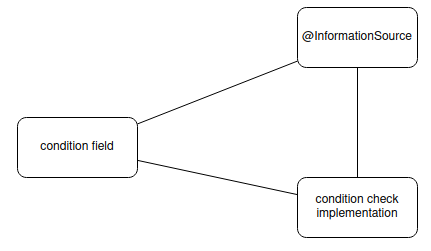
\includegraphics[width=0.75\linewidth]{./figures/condition-triplet-pattern}
    \caption{Geneic illustration of the triplet pattern}
    \label{fig:condition-triplet-pattern}
\end{figure}

Figure \addref and figure \addref display concrete instances of this pattern.


\begin{figure}
    \centering
    \begin{subfigure}[b]{0.45\linewidth}
        \centering
        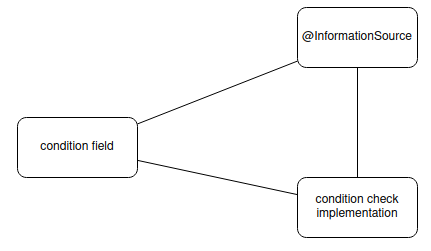
\includegraphics[width=\linewidth]{./figures/condition-triplet-pattern}
        \caption{Condition Triplet pattern instance 1}
        \label{fig:condition-triplet-pattern-instance-1}
    \end{subfigure}
    % Adjust or remove the space between figures as needed
    \hspace{5mm} % This adds a bit of horizontal space between the figures
    \begin{subfigure}[b]{0.45\linewidth}
        \centering
        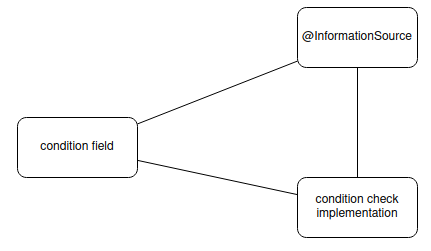
\includegraphics[width=\linewidth]{./figures/condition-triplet-pattern}
        \caption{Condition Triplet pattern instance 2}
        \label{fig:condition-triplet-pattern-instance-2}
    \end{subfigure}
    \label{fig:coffee}
\end{figure}







\chapter{Results}\label{ch:results}
%This chapter demonstrates the performance of the billing framework applied to realistic treatment cases.
In this chapter, we apply the framework to treatment cases developed with the assistance of billing experts.
The cases represent realistic treatments that are likely to occur in clinical practice and that are, from a billing perspective, interesting and non-trivial.
Billing experts at \AV subsequently validated the quality of the results.
The framework proved largely capable of generating accurate billings.
However, we also identified limitations of the framework in the results and during the rule-writing process.

This chapter is structured as follows:
Firstly, section \ref{sec:experimental-rule-base} introduces the rules we preloaded the Billing Server with before performing the actual experiments.
In this work, we can only present a limited set of rules.
A realistic rule-base used in production would need at least hundreds of rules even with tight restrictions to specific medical areas.

An additional purpose of this section is to further illustrate the usage of the rule features of \RL.
As a side note, the presented rules are a subset of the rule base that will be employed in production by \AV.
Secondly, in the next sections we introduce the patient cases which we generate billing codes.
This involves patient background information, history and outcomes that are part of the patient anamnesis and physical examinations.
Applied medical procedures also characterize these treatments.
For each treatment, we compare the actually derived codes with the expected ones determined by the billing experts.

\section{Experimental Rule Base}\label{sec:experimental-rule-base}

\subsection{GOÄ Examination Code Rules}\label{subsec:examination-code-rules}
Examination Codes are frequently used codes that apply to provided physical examinations.
They primarily base on the existence of physical examination blocks in the treatment.
We consider the following codes in the experiments.

\paragraph{\goa{5: Symptom-related examination}}
\goa{5} applies to examinations the practitioner provides using simple medical tools.
According to the GOÄ, typical examinations that fall into that category are inspections, palpations, percussions and reflex testings.
The following rule checks for an existing examination of that type.
\lstinputlisting[
language=json,
style=json,
caption={\goa{5: Examination to determine the whole body status, including documentation if necessary}}
label={lst:goae-5-rule}
]{code/rules/experiments/goae-base-rules-5.json}

\paragraph{\goa{6}}
\goa{6} applies to examinations of at least on of the following organ systems:
\begin{itemize}
    \item All sections of the eye
    \item The entire ENT (ear, nose, throat) area
    \item The stomatognathic system
    \item The kidneys and urinary tract
    \item Examination to determine a complete vascular status
\end{itemize}
For the case of simplicity, the code snipped illustrating the rule for \goa{6} omits a few less interesting details.
\goa{6} further requirements on the provided examination \cite{bruck1998kommentar}.
For example, an eye related examination must striclty cover both eyes.
The same must hold for the ears, if the practitioner provided an ENT examination.
The rule implements this by not only requiring the existence of blocks, as it does for the \code{visualAcuity} and \code{oculomotorSkills},
but also expressing conditions on nested objects in the blocks.
For example, it specifies the existence of a \code{pupilLeft} and \code{pupilRight} block inside the \code{pupilsAndLightReaction} physical examination block.
The rule specifies an equivalent expression for \code{earsAndMastoidPalpation}.

\lstinputlisting[
language=json,
style=json,
caption={\goa{6}}
label={lst:goae-6-rule}
]{code/rules/experiments/goae-base-rules-6.json}


\lstinputlisting[
language=json,
style=json,
caption={\goa{6: Complete physical examination of at least one of the following organ systems: all eye sections, the entire ENT area, the stomatognathic system, the kidneys and urinary tract (in men, including the male genital organs if necessary) or examination to determine a complete vascular status - including documentation, if necessary}}
label={lst:goae-5-rule}
]{code/rules/experiments/goae-base-rules-5.json}


\paragraph{\goa{7}}
\goa{7} applies to detailed physical examinations of at least one of the following entire organ system:
\begin{itemize}
    \item Skin organ
    \item Support and movement organs
    \item Chest organs
    \item Abdominal organs
    \item Female genital tract
\end{itemize}
For the case of simplicity, the following rule only considers the skin and the support and movement organs.
The omitted organ systems are not relevant for the experimental treatment cases.
\lstinputlisting[
language=json,
style=json,
caption={\goa{7: Complete physical examination of at least one of the following organ systems: the entire skin organ, the supporting and locomotor organs, all breast organs, all abdominal organs, the entire female genital tract (including kidneys and urinary tract, if applicable) - including documentation, if applicable -}}
label={lst:goae-7-rule}
]{code/rules/experiments/goae-base-rules-7.json}


\paragraph{\goa{8: Examination to determine the whole body status, including documentation if necessary}}
According to its description in the GOÄ \cite{hermanns2015ebm}, it is applicable if the doctor provided the following types of examinations:
\begin{itemize}
    \item Examinations of the skin
    \item Examinations of the visible mucous membranes
    \item Examinations of the breast or abdominal organs
    \item Examinations of the supporting and movement organs
    \item Orienting neurological examination
\end{itemize}
We need to conjugate the existence of all those five examinations to check if \goa{8} is applicable.
We can easily use the logical tree feature presented in \addref to implement this as follows.
The rule assumes that an examination of the skin is present if the practitioner has entered data into the \code{skinChangeExaminations} block as part of the physical examination stage.
It assumes that an examination of the supporting and movement organs is present if the practitioner has entered data into the \code{mobilityTestCervicalSpine}, the \code{mobilityTestThoracicSpine} or the \code{mobilityTestLumbarSpine} block.
Writing rules for examination codes like \goa{8} requires us to define a mapping between the anamnesis or physical examination blocks from the \AV data model and the concrete examinations required by the rule.

\lstinputlisting[
Language=json,
style=json,
caption={\goa{8: Examination to determine the whole body status, including documentation if necessary}}
label={lst:goae-8-rule}
]{code/rules/experiments/goae-base-rules-8.json}

\paragraph{\goa{11: Digital examination of the rectum and/or prostate}}
This code applies for treatments with an examination of the rectum or prostate.
This condition translates to the existence of a \code{digitalRectalExamination} or a \code{prostateExamination} block.

\lstinputlisting[
Language=json,
style=json,
caption={GOÄ 11}
label={lst:goae-11-rule}
]{code/rules/experiments/goae-base-rules-11.json}



%Note that we use the \code{physicalBlocks} field to express conditions on physical examination blocks.
%The rule represents each of the mentioned organ systems as a child node of the root node.
%The root node applies an \code{AND} operation to all its sub-children.
%Each sub-child represents one of the organ systems required by \goa{8}.
%The \AVS does not directly define an organ systems examination
%However, we can flexibly define an organ system examination by a logical tree of required physical blocks.
%This rule defines a skin examination to be present if a \code{skinTurgor}, a \code{skinColor}, a \code{skinThickness} or a \code{skinChangeExamination} block is present.
%We can represent the rest of the organ systems in a similar way using the logical tree pattern.
%Additionally there is already a respective single block for the orienting neurological examination.
%
%Note that the rule checks only for existence of examination blocks and does not impose any field conditions.


\subsection{Special GOÄ Consultation Code Rules}\label{subsec:special-consultation-code-rules}

\paragraph{\goa{1: Advice – also via telephone}}\label{par:goa-1}
\goa{1} is one of the most commonly used codes in the GOÄ.
It is applicable for a conversation between patient and doctor at the beginning of the visit that takes at most 10 minutes.
This type of conversation happens typically as part of the anamnesis.

Unfortunately, this is where the billing framework as well as the \AVS reaches its limits.
It is practically impossible to automatically track the time of the initial conversation between patient and practitioner.
One idea could be to track the time passed between the practitioner entering the anamnesis page and moving on to the physical examination page in the front-end.
This is, however, highly unreliable as doctors often enter the data into the software at the very end of the treatment.
One slightly less user-friendly way to solve is to make the user explicitly enter the duration of the anamnesis.
The current version of the \AVS does not offer this possibility, making reliably deriving \goa{1} not possible.
The user needs to add this code manually.

\paragraph{\goa{3: In-depth advice that goes beyond the usual level – also by telephone –}}
\goa{3} is similar to \goa{1} but applies to doctor patient consultations that take longer than 10 minutes.
Again, we have the same issue here as in \ref{par:goa-1} and are not able to automatically derive it.

\subsection{GOÄ Surcharges}\label{subsec:goa-surcharges}
The GOÄ defines surcharges that are easily missed out in praxis.
Section \ref{sec:surcharges} covers them in details where we also mention that surcharges have tight exclusion rules.
These exclusions are already part of the structured data in the GOÄ catalog, making the usage of the \code{excludedCodes} fields here obsolete.
The codes from \goa{401} up to \goa{410} are surcharges as well, but are not relevant for the experimental treatments provided by \AV.

\lstinputlisting[
language=json,
style=json,
caption={\goa{A: Surcharge for services provided outside office hours}}
label={lst:goae-A-rule}
]{code/rules/experiments/goae-base-rules-A.json}

\lstinputlisting[
language=json,
style=json,
caption={\goa{B: Surcharge for services provided outside office hours between 8 p.m. and 10 p.m. or 6 a.m. and 8 a.m}}
label={lst:goae-8-rule}
]{code/rules/experiments/goae-base-rules-B.json}

\lstinputlisting[
language=json,
style=json,
caption={\goa{C: Surcharge for services provided between 10 p.m. and 6 a.m}}
label={lst:goae-C-rule}
]{code/rules/experiments/goae-base-rules-C.json}

\lstinputlisting[
language=json,
style=json,
caption={\goa{D: Surcharge for services provided on Saturdays, Sundays or public holidays}}
label={lst:goae-D-rule}
]{code/rules/experiments/goae-base-rules-D.json}

The following surcharges are applicable to patients younger than 4 years old if one of the required GOÄ codes are present.

\lstinputlisting[
language=json,
style=json,
caption={\goa{K1: Surcharge to the benefits according to numbers 45, 46, 48, 50, 51, 55 or 56 for children up to the age of 4}}
label={lst:goae-K1-rule}
]{code/rules/experiments/goae-base-rules-K1.json}

\lstinputlisting[
language=json,
style=json,
caption={\goa{K2: Surcharge for examinations according to numbers 5, 6, 7 or 8 for children up to the age of 4}}
label={lst:goae-K2-rule}
]{code/rules/experiments/goae-base-rules-K2.json}

\goa{E} is a surcharge for services that require special urgency.
A patient experiencing severe pain often necessitates urgent medical intervention.
In these situations, the doctor documents the patient's pain level.
The pain level can be seen as an indicator for the urgency of the treatment and therefore used as a hint for \goa{E}, which is a surcharge applicable for urgent treatments.
\lstinputlisting[
Language=json,
style=json,
caption={\goa{E: Surcharge for services requiring special urgency}}
label={lst:goae-E-rule}
]{code/rules/experiments/goae-base-rules-E.json}


\subsubsection{Procedure GOÄ Rules}

The procedure GOÄ rules are primary based on the work of Dr. Sarah Bojko, who has a deep understanding of the specification of the procedure available in the \AVS.

\paragraph{1530 and 1533}
\goa{1530: Examination of the larynx with the laryngoscope} and \goa{1533: Floating or supporting laryngoscopy, each as an independent service} are both codes referring to a laryngoscopy procedure.
The \code{LaryngoscopyMsg} block represents this procedure and has a boolean field \code{floatingOrSupportedLaryngoscopy}.
Both rules check for the existence of a laryngoscopy and the required value of the \code{floatingOrSupportedLaryngoscopy} boolean field.
Only one of both rule can match at one time.
\lstinputlisting[
language=json,
style=json,
caption={Rules for \goa{1530} and \goa{1533}}
label={lst:goae-1530-1533-rules}
]{code/rules/experiments/goae-procedure-rule-1530-1533.json}

\paragraph{255}
\goa{255: Injection, intra-articular or perineural} refers to a spine infiltration represented by the \code{spineInfiltration} procedure block.
Subsection \ref{subsubsec:quantity-derivation-from-procedure-information} introduces the concept of quantity functions using the example of the spine infiltration.

The following rule matches if a spineInfiltration exists followed by the computation the quantity of its conclusion code \code{255}.
Code snippet \ref{lst:spineInfiltration} illustrates its protobuf representation, the field paths used in the rule must comply with.

\lstinputlisting[
    language=json,
    style=json,
    caption={Rule for \goa{255: Injection, intra-articular or perineural}}
    label={lst:goae-255-rule}
]{code/rules/experiments/goae-procedure-rule-255.json}

The spine infiltration block has a localization field for all possible injection localizations in the human spine,
making the object in the data model quite extensive.
The rule specifies a field evaluation sub-function for each of those localization fields.
The actual rule consists of more than 200 lines of codes,
which is why we can only include a small section of it in the code snippet.
\lstinputlisting[
    language=json,
    style=json,
    caption={\goa{E: Surcharge for services requiring special urgency}}
    label={lst:goae-1530-rule}
]{code/rules/experiments/goae-procedure-rule-1530-1533.json}

\paragraph{460 and 461}
\goa{460: Combination anesthesia with mask, device - also insufflation anesthesia -, up to one hour}
and \goa{461: Combination anesthesia with mask, device - also insufflation anesthesia - every additional half hour} are two GOÄ codes that refer to the same service but cover different time spans.
Subsection \goa{subsec:quantity-derivation-from-durations} already introduces this type of duration interconnections between GOÄ codes in more details.

\lstinputlisting[
language=json,
style=json,
caption={\goa{6}}
label={lst:goae-6-rule}
]{code/rules/experiments/goae-procedure-rule-460.json}

Code \code{460} holds if a \code{generalAnesthesia} block with the required fields exists.
Code \code{461} holds if a \code{generalAnesthesia} block with the required fields exists and the procedure has a duration of at least 60 minutes.
In this case, the quantity of \code{461} is equal to the number of 30-minute-spans that subsequently follow the first 60 minutes.
The quantity of \code{461} must ignore the first two 30-minute-spans, which is why the quantity function counts the number of commenced 30-minute-spans, subtracting the first two.
Adding a constant of \code{-2} to the procedure duration expression in the quantity function implements this logic.

\paragraph{473 and 474}
\goa{473: Induction and monitoring of continuous subarachnoid spinal anesthesia (lumbar anesthesia) or epidural (epidural) anesthesia with catheter, lasting up to five hours}
and
\goa{474: Induction and monitoring of continuous subarachnoid spinal anesthesia (lumbar anesthesia) or epidural (epidural) anesthesia with catheter, lasting more than five hours}
Are also two anesthesia billing codes that refer to the same type of service but distinguish between durations
The rules in the following code snippet implement both billing conditions
Code \code{473} applies if the practitioner provided a \code{neurexialAnesthesia} procedure with one of the required procedure types and the duration took less than five hours.
Code \code{474} applies for the case when the same procedure takes more than five hours.

\lstinputlisting[
language=json,
style=json,
caption={\goa{473 and 474}}
label={lst:goae-6-rule}
]{code/rules/experiments/goae-procedure-rule-473-474.json}


\subsection{Multiplier Justification Rules}\label{subsec:multiplier-justification-rules}
Sections \ref{sec:billing-multipliers} and \ref{sec:multiplier-justifications} introduce the concept of billing multipliers in private treatments.
Multipliers apply to existing GOÄ codes.
However, they require provable justifications and must rely on facts in the treatment data.
As multiplier justifications are neither standardized nor pre-defined by any authority,
part of this work was to collect commonly used multiplier justifications.
Thanks to the medical experts at \AV, I received access to medical documents that contained multiplier justifications used in the Dermato Oncology department of the LMU.
Many of the following rules implement those justifications.
As mentioned in section \ref{sec:language-design-workflow}, I participated in the PVS Seminar, where I received more information about possible multiplier justifications.
As described in subsection \ref{subsec:the-target-code-field}, Multiplier justifications can be target-specific or generally applicable.

\lstinputlisting[
    language=json,
    style=json,
    caption={\goa{Multiplier Justification refering to communication issues}},
    label={lst:mj-communication-rule}
]{code/rules/experiments/justification-rule-communication.json}


\lstinputlisting[
language=json,
style=json,
caption={\goa{Multiplier Justification refering to issues caused by the patient's current drug abuse}},
label={lst:mj-cdrug-rule}
]{code/rules/experiments/justification-rule-multimorbidity.json}


\subsubsection{Procedure-specific and duration-related multiplier justifications}
Procedures often take longer than expected, which can be the case due to unforeseen complications and issues.
The following rule list shows the generic pattern used for procedure-specific and duration-related multiplier justifications.

%\lstinputlisting[
%    language=json,
%    style=json,
%    caption={\goa{Generic procedure duration multiplier justification rule}},
%    label={lst:goae-K2-rule}
%]{code/rules/experiments/goae-base-rules-K2.json}

\todo{add rules}

The rule base contains implementations of that pattern for each of the procedures that the system currently supports.
Note that the rule only checks for the existence of the respective procedure block.
We use the special block conditions \code{\$minDuration} and \code{\$maxDuration} to make the rule only match if the duration of the procedure is within the specified interval.
Each procedure may have multiple duration-related justification rules, covering another time interval and multiplier value.

%\lstinputlisting[
%    language=json,
%    style=json,
%    caption={\goa{E: Surcharge for services requiring special urgency}},
%    label={lst:goae-E-rule}
%]{code/rules/experiments/goae-base-rules-E.json}


\section{GOÄ results}\label{sec:goa-results}

\subsection{Patient Case 1: Multiple spine infiltrations due to back pain with obesity}\label{subsec:patient-a---multiple-spine-infiltrations-due-to-backpain-with-obesity}
The patient is a 57-year-old female suffering from chronic back pain.
The patient has two other visits with the same issue concerning back pain and was previously diagnosed with the so-called facet syndrome (\mete{M47.2}).

\paragraph{Anamnesis}
In the anamnesis stage the

\paragraph{Physical Examination}
In the physical examination stage the doctor conducts several examinations.
The doctor firstly checks for neurological issues.
She performs a orienting neurological examination and examines the posture and stand of the patient.
In both examinations she does not detect anything conspicuous.
Next, she examines the patient's spine mobility.
She performs a mobility test for the thoracic spine (\code{MobilityTestThoracicSpineBlock}) and the lumbar spine (\code{mobilityTestLumbarSpineBlock}) and detects existing mobility issues.
Additionally, the practitioner notes down the patient's nutrition status, leading to the results that the patient suffers from obesity.

\paragraph{Procedures}
The previous stages have revealed chronic back pain due to a diagnosed facet syndrome, missing neurological issues and obesity.
This is why she decides to perform non-operative and conservative treatment, namely a spine infiltration.
A spine infiltration is applicable to chronic and acute back pain issues to reduce the pain.
As the patient suffers from the facet syndrome, the doctor decides to perform facet injections in the spine infiltration procedure.
In a Facet Infiltration, the performer makes direct injections into the spine joints instead of the surrounding muscles.
She performs the following injections:
\begin{itemize}
    \item one nerve root injection on the left side of TH2 in the thoracic spine
    \item one facet injection on both sides of TH6 in the thoracic spine
    \item one facet injection on the right side of L1 in the lumbar spine
\end{itemize}

\paragraph{Difficulties and Inconveniences}
Overweight individuals have a thicker layer of subcutaneous fat, making locating veins, muscles and joins more difficult.
Additionally, doctors may need special syringes with longer needles to penetrate the fat layer to reach the underlying joint.


\subsubsection{Expected Results}
The billing for the treatment should compensate the doctor for the performed examinations and each single spine infiltration.
The challenging condition of the spine infiltration caused by the patient's nutrition status is a valid justification for a multiplier applied to the spine infiltration billing code.
The physical examination consisted of an orienting neurological examination and multiple spine mobility tests.


\subsubsection{Actual Results}
The framework was unable to derive \goa{1} due to the issues already described in subsection \ref{subsec:special-consultation-code-rules}.

The framework successfully derived \goa{8}, covering all the mobility tests and the neurological examination.
Other examination codes failed due to missing blocks.

The framework derived \goa{255} with the correct quantity of four.
Rule \ref{lst:goae-255-rule} checked for the existence of a \code{spineInfiltration} block which was given in the documentation.
The rule engine also computed the quantity by evaluating each child function for the corresponding localization field in the \code{spineInfiltration} object and returned the correct quantity.
Additionally, the framework detected the patient's obesity as a challenging factor for the infiltration,
sucessfully deriving the multiplier justification \addref.




%spine infiltration
%-> 4 spine infiltrations -> 4 x GOÄ 255
%multipliers:
%Erhöhter Aufwand bei SpineInfiltration aufgrund von Übergewicht

%Codes:
%1 x GOÄ 1
%1 x GOÄ 8
%4 x GOÄ 255 mit multiplier



\subsection{Patient Case 2: Injury of child}\label{subsec:patient-case-2:-anesthesia-for-birth}
The patient is a four-years-old boy that came to the doctor due to an injury while playing soccer.

Patient B - Körperliche Untersuchung mit Kind -> Fußball verletzung


- männlich


Anamnese:
? sports block fussball

examination:
->

GOÄ 1
GOÄ 4
GOÄ 7
GOÄ K1

\subsection{Patient Case 3: Anesthesia Provision For Birth}\label{subsec:patient-case-3:-anesthesia-for-birth}
The patient is a 32-year-old woman and is currently about to give birth on a Wednesday at 3 am.
It is common practice to create two bills for birth, one for the anesthetist and another for the gynecologist.
The treating anesthetist is not a doctor but a care professional.
This scenario covers the billing for the anesthesia.
The current version of the \AVS does not cover birth treatments.
The patient did not register as a native German speaker but has sufficient English capabilities.

\paragraph{Anamnesis}
The treatment starts with a short introductory conversation between the patient and the anesthetist.
This involves details about the anesthesia and the patient's current and previous pregnancies.
Additionally, the practitioner documents the patient's high level of pain.
The practitioner enters a pain severity of 8 into the software.

\paragraph{Physical Examination}
Blood oxygen monitoring is an essential part of an anesthesia procedure to ensure the patient's safety, which happens during the physical examination stage.
The doctor makes a single pulse oximetry measurement of 95 and documents the results in a \code{Respiration} block.

\paragraph{Procedures}
Finally, the anesthetist performs a so-called spinal anesthesia with catheter technology.
The practitioner documents the details in the corresponding \code{neurexialAnesthesia} procedure block.
Finally, the anesthetist performs a so-called spinal anesthesia with catheter technology.
The practitioner documents the details in the corresponding \code{neurexialAnesthesia} procedure block.
The anesthesia will be kept stable during the entire birth and will last for 11.5 hours.

\paragraph{Difficulties and Inconveniences}
The requirement to communicate in english during such a critical treatment is considerable as a challenging condition for the practitioners.

\subsubsection{Expected Results}
The introductory conversation in the anamnesis stage took longer than 10 minutes, making \goa{1} applicable.
The system should derive \goa{614: Transcutaneous measurement(s) of oxygen partial pressure} for measuring the pulse oximetry during the anesthesia.
Additionally, the framework should suggest \goa{474} for the actual anesthesia performed before the birth.
The framework must not confuse it with \goa{473}, which applies to equal anesthesia services that take less than 5 hours.
Due to the critical nature of birth and the pain experienced by the patient, this anesthesia treatment is highly urgent, justifying the application of \goa{E: Surcharge for urgently requested and immediate execution}.
Additionally, the treatment happens at an inconvenient time at 3 am during the week,
making \goa{D: Surcharge for services provided between 10 pm and 6 am} applicable.
Additionally, the framework should suggest an appropriate multiplier justification that compensates for the requirement to communicate in English.

\subsubsection{Actual Results}
The framework could not derive \goa{1} due to the issues already described in subsection \ref{subsec:special-consultation-code-rules}.
It successfully derived a multiplier justification for the communication problems.
However, this multiplier should apply to a consultation service such as \goa{1}, which the user must manually add.

A \code{neuraxialAnesthesiaMsg} block was also part of the treatment, triggering rules in listing \ref{lst:goae-473-474-rule}.
Both rules check the procedure duration of \code{neuraxialAnesthesiaMsg}.
As the anesthesia lasts 11.5 hours, the framework correctly rejected \code{473} and accepted \code{474}.

Code \code{614} matches due to the respiration documentation.
Rule \ref{lst:goae-614-rule} checks for the presence of a respiration measurement that includes a pulse oximetry measurement.
The anesthetist performed a single measurement with an oximetry value of 95, which matches the rule.

The framework also derived the \goa{E} surcharge applicable for urgent treatment.
Rule \ref{lst:goae-E-rule} matched due to the high pain documented in the \code{pain} block during anamnesis.
The anesthesist documented a pain score of 8, which is greater than the minimum limit of 6 specified in the rule.

The treatment occurs at 3 am on a Wednesday night, outside any office hours.
This triggers surcharges \goa{A} and \goa{C}, which mutually exclude themselves.
The conflict resolution algorithm chose \goa{C} (320 points) over \goa{A} (70 points).
This results in the following bill.

%Codes:
%1 x GOÄ 1
%1 x GOÄ 614 (due to respiration)
%1 x GOÄ 473 (anesthesia)
%1 x GOÄ E (surcharge for urgency)
%1 x GOÄ C (surcharge for )


%-> respiration block mit pulseOximetry > 94


Patient B - Körperliche Untersuchung mit Kind -> Fußball verletzung

- hat sprachprobleme
- männlich


Anamnese:
? sports block fussball

examination:
->

GOÄ 1
GOÄ 4
GOÄ 7
GOÄ K1


\section{Discussion}\label{sec:discussion}

I want to express the following:

the experiments have shown that the framework and the rule language successfully derive most codes with a correct quantity.
however, the results have also shown concrete limitations.





As concluded in section \ref{sec:common-issues-with-modern-billing-automation-products} the central issue for automatic billing generation is the requirement for structured data.
The upper bound for the quality of the generation results is the completeness of the structured data that the framework has access to.

The reason for the missing billing codes in the previous experiments are condition features that the \RL currently does not provide.


One class code types is the set of services that focus on the patient-practitioner contact.
This includes \goa{1} and \goa{3}, \goa{4}, \goa{21} and \todo{orther}.
Rules in this code class have a high variety in used condition type.
Duration-related conditions are of high importance for this code class.
For example, we have seen that \goa{1} and \goa{3} rely on the anamnesis duration.
There are other codes and use cases for durations of specific stages and actions during a treatment, but those durations are unfortunately not part of the structured data.
The reason for that is that durations are not easily trackable in practice.
Measuring the time of an anamnesis, would require the front-end to start a timer when the anamnesis starts and to stop it when it finishes.
According to the engineers at \AV, we unfortunately cannot rely on specific user actions in the UI.
A user does not necessarily switch from the anamensis to the physical examination stage at the very moment when the anamnesis actually finishes.
Making the user manually enter durations into the user interface is neither a practical or user-friendly solution.
Durations the only information sources missing in the \AV data model.
\goa{21}, \goa{22}, \goa{23}, \goa{27}, \goa{30} are all consultation services that rely on consultation details that the \AV currently does not track,
either because tracking them automatically is infeasible or the current software version simply does not cover these service areas.




Another class of billing codes are examination related codes.
We have proven that the framework is indeed capable of successfully deriving this class of codes.
In this case, checking for existences of blocks using logical combinations has turned out to be extremely useful here.
This also requires a correct mapping of blocks to the examinations mentioned in the rule.

Finally, we have the class of billing codes relating to specific procedures and which represent the overwhelming majority of the GOÄ.
Writing rules for these codes is comparably simple.
Most of the rules in this class purely rely on a specific procedure which can be expressed using the \requiredProcedure condition.
The future production rule-base will probably contain multiple groups of procedure-related rules.
Each group references a procedure defined in the \AV model.
Each rule in this group checks has a slightly different conclusion code and checks for other conditions in the procedure block.


In cases where codes cannot be automatically derived, users need to manually add them in the billing stage.
As long as this issue persists, the billing framework should not be considered to generate a full and perfectly acceptable billing,
but rather a set of suggestions that might require manual updates.









\appendix{}

\microtypesetup{protrusion=false}
\listoffigures{}
\listoftables{}
\microtypesetup{protrusion=true}
\printbibliography{}

\end{document}
